% Options for packages loaded elsewhere
\PassOptionsToPackage{unicode}{hyperref}
\PassOptionsToPackage{hyphens}{url}
%
\documentclass[
]{book}
\usepackage{lmodern}
\usepackage{amsmath}
\usepackage{ifxetex,ifluatex}
\ifnum 0\ifxetex 1\fi\ifluatex 1\fi=0 % if pdftex
  \usepackage[T1]{fontenc}
  \usepackage[utf8]{inputenc}
  \usepackage{textcomp} % provide euro and other symbols
  \usepackage{amssymb}
\else % if luatex or xetex
  \usepackage{unicode-math}
  \defaultfontfeatures{Scale=MatchLowercase}
  \defaultfontfeatures[\rmfamily]{Ligatures=TeX,Scale=1}
\fi
% Use upquote if available, for straight quotes in verbatim environments
\IfFileExists{upquote.sty}{\usepackage{upquote}}{}
\IfFileExists{microtype.sty}{% use microtype if available
  \usepackage[]{microtype}
  \UseMicrotypeSet[protrusion]{basicmath} % disable protrusion for tt fonts
}{}
\makeatletter
\@ifundefined{KOMAClassName}{% if non-KOMA class
  \IfFileExists{parskip.sty}{%
    \usepackage{parskip}
  }{% else
    \setlength{\parindent}{0pt}
    \setlength{\parskip}{6pt plus 2pt minus 1pt}}
}{% if KOMA class
  \KOMAoptions{parskip=half}}
\makeatother
\usepackage{xcolor}
\IfFileExists{xurl.sty}{\usepackage{xurl}}{} % add URL line breaks if available
\IfFileExists{bookmark.sty}{\usepackage{bookmark}}{\usepackage{hyperref}}
\hypersetup{
  pdftitle={Statistics with jamovi},
  pdfauthor={Dana Wanzer},
  hidelinks,
  pdfcreator={LaTeX via pandoc}}
\urlstyle{same} % disable monospaced font for URLs
\usepackage{longtable,booktabs}
% Correct order of tables after \paragraph or \subparagraph
\usepackage{etoolbox}
\makeatletter
\patchcmd\longtable{\par}{\if@noskipsec\mbox{}\fi\par}{}{}
\makeatother
% Allow footnotes in longtable head/foot
\IfFileExists{footnotehyper.sty}{\usepackage{footnotehyper}}{\usepackage{footnote}}
\makesavenoteenv{longtable}
\usepackage{graphicx}
\makeatletter
\def\maxwidth{\ifdim\Gin@nat@width>\linewidth\linewidth\else\Gin@nat@width\fi}
\def\maxheight{\ifdim\Gin@nat@height>\textheight\textheight\else\Gin@nat@height\fi}
\makeatother
% Scale images if necessary, so that they will not overflow the page
% margins by default, and it is still possible to overwrite the defaults
% using explicit options in \includegraphics[width, height, ...]{}
\setkeys{Gin}{width=\maxwidth,height=\maxheight,keepaspectratio}
% Set default figure placement to htbp
\makeatletter
\def\fps@figure{htbp}
\makeatother
\usepackage[normalem]{ulem}
% Avoid problems with \sout in headers with hyperref
\pdfstringdefDisableCommands{\renewcommand{\sout}{}}
\setlength{\emergencystretch}{3em} % prevent overfull lines
\providecommand{\tightlist}{%
  \setlength{\itemsep}{0pt}\setlength{\parskip}{0pt}}
\setcounter{secnumdepth}{5}
\usepackage{booktabs}

\newenvironment{danger}
    {
    \hline\\
    }
    { 
    \\\\\hline
    }
    
\newenvironment{warning}
    {
    \hline\\
    }
    { 
    \\\\\hline
    }
    
\newenvironment{info}
    {
    \hline\\
    }
    { 
    \\\\\hline
    }
    
\newenvironment{try}
    {
    \hline\\
    }
    { 
    \\\\\hline
    }
\ifluatex
  \usepackage{selnolig}  % disable illegal ligatures
\fi
\usepackage[]{natbib}
\bibliographystyle{apalike}

\title{Statistics with jamovi}
\author{Dana Wanzer}
\date{Last Update: 2020-11-04}

\begin{document}
\maketitle

{
\setcounter{tocdepth}{1}
\tableofcontents
}
\hypertarget{welcome}{%
\chapter*{Welcome}\label{welcome}}
\addcontentsline{toc}{chapter}{Welcome}

This is the website for PSYC 290 and PSYC 790 at the University of Wisconsin-Stout, taught by Dana Wanzer. These resources are aimed at teaching you how to use jamovi and null hypothesis significance testing (NHST) to answer research questions.

This website is \textbf{free to use} and is licensed under a Creative Commons BY-SA (CC BY-SA) license version 4.0. This means you are free to \textbf{share} (i.e., copy and redistribute the material in any medium or format) and \textbf{adapt} (i.e., remix, transform, and build upon the material for any purpose, even commercially), provided that you \textbf{attribute} these resources by citing me, indicating if changes were made and you \textbf{share alike} (i.e., if you adapt, you must distribute your contributes under the same license as the original).

Portions of this book may have been adapted from ``\href{http://www.learnstatswithjamovi.com}{Learning statistics with jamovi: A tutorial for psychology students and other beginners}'' by Danielle J. Navarro and David R. Foxcroft, version 0.70. Furthermore, the template and style of this book is from \href{https://psyteachr.github.io/book-template/setup.html}{PsyTeachR}.

\hypertarget{introduction}{%
\chapter{Introduction}\label{introduction}}

This chapter will walk you through how this website/book works.

\hypertarget{quiz-questions}{%
\section{Quiz Questions}\label{quiz-questions}}

Throughout this website, there will be questions to help you test your knowledge. When you type in or select the correct answer, the dashed box will change color and become solid.

For example:

\begin{itemize}
\item
  What is 2+2?
\item
  We attend the University of Wisconsin- Stout Madison Green Bay
\item
  True or false: Statistics is awesome. TRUE FALSE
\end{itemize}

\hypertarget{errors-and-mistakes}{%
\section{Errors and mistakes}\label{errors-and-mistakes}}

I am human, therefore I err. If you find an error in the textbook or something you think might be a mistake, please let me know ASAP so I can update this for everyone else. Let me know which section you find the error or mistake in and what the error or mistake is. For example, if there was an error here you could say, ``There was an error in 1.2 that the first sentence should really be `To err is human.'\,''

\hypertarget{part-t-tests}{%
\part{t-tests}\label{part-t-tests}}

\hypertarget{independent-t-test}{%
\chapter{Independent t-test}\label{independent-t-test}}

\hypertarget{what-is-the-independent-t-test}{%
\section{What is the independent t-test?}\label{what-is-the-independent-t-test}}

The independent t-test is used to test the difference in our dependent variable between two different groups of observations. Our grouping variable is our independent variable. In other words, we use the independent t-test when we have a research question with a \textbf{continuous dependent variable} and a \textbf{categorical independent variable with two categories in which different participants are in each category}.

The independent t-test is also called the independent samples t-test and the Student's t-test. I will use these terms interchangeably.

There are three different types of alternative hypotheses we could have for the independent t-test:

\begin{enumerate}
\def\labelenumi{\arabic{enumi}.}
\item
  \textbf{Two-tailed}

  \begin{itemize}
  \tightlist
  \item
    \(H_1\): Group 1 has a different mean than Group 2.
  \item
    \(H_0\): There is no difference in means between the two groups.
  \end{itemize}
\item
  \textbf{One-tailed}

  \begin{itemize}
  \tightlist
  \item
    \(H_1\): Group 1 has a greater mean than Group 2.
  \item
    \(H_0\): The mean for Group 1 is less than or equal to the mean for Group 2.
  \end{itemize}
\item
  \textbf{One-tailed}

  \begin{itemize}
  \tightlist
  \item
    \(H_1\): Group 1 has a small mean than Group 2.
  \item
    \(H_0\): The mean for Group 1 is greater than or equal to the mean for Group 2.
  \end{itemize}
\end{enumerate}

\hypertarget{data-set-up}{%
\section{Data set-up}\label{data-set-up}}

To conduct the independent t-test, we first need to ensure our data is set-up properly in our dataset. This requires having two columns: one with our continuous dependent variable and one indicating which group the participant is in. Each row is a unique participant or unit of analysis. Here's what example data may look like if we were testing for differences in a test score by students in my fall or spring semesters of this course:

\begin{longtable}[]{@{}llr@{}}
\caption{Example data for the independent t-test}\tabularnewline
\toprule
ID & Semester & TestScore\tabularnewline
\midrule
\endfirsthead
\toprule
ID & Semester & TestScore\tabularnewline
\midrule
\endhead
1 & Fall & 86\tabularnewline
2 & Fall & 80\tabularnewline
3 & Fall & 75\tabularnewline
4 & Fall & 79\tabularnewline
5 & Fall & 82\tabularnewline
6 & Spring & 84\tabularnewline
7 & Spring & 90\tabularnewline
8 & Spring & 72\tabularnewline
9 & Spring & 75\tabularnewline
10 & Spring & 81\tabularnewline
\bottomrule
\end{longtable}

In the example data above, what is your \textbf{independent variable}? ID Semester TestScore

In the example data above, what is your \textbf{dependent variable}? ID Semester TestScore

\hypertarget{the-math-behind-the-independent-t-test}{%
\section{The math behind the independent t-test}\label{the-math-behind-the-independent-t-test}}

\begin{info}
If the math below makes your eyes glaze over, you can skip it. This is
presented for those who find it useful to understand the math behind the
statistics to help understand what's happening.
\end{info}

The basic math of the independent t-test the mean difference divided by the pooled standard error.

\(t = \frac{\bar{X}_1 - \bar{X}_2}{SE({\bar{X}_1 - \bar{X}_2})}\)

The denominator of the equation is more difficult to calculate and depends on whether the sample size between groups is equal.

\hypertarget{assumptions}{%
\section{Assumptions}\label{assumptions}}

As a parametric test, the independent t-test has the same assumptions as other parametric tests:

\begin{enumerate}
\def\labelenumi{\arabic{enumi}.}
\item
  The dependent variable is \textbf{normally distributed}
\item
  Variances in the two groups are roughly equal (i.e., \textbf{homogeneity of variances})
\item
  The dependent variable is \textbf{interval or ratio} (i.e., continuous)
\item
  Scores are \textbf{independent} between groups
\end{enumerate}

We cannot \underline{test} the third and fourth assumptions; rather, those are based on knowing your data.

However, we can and should test for the first two assumptions. Fortunately, the independent samples t-test in jamovi has two check boxes under ``Assumption Checks'' that lets us test for both assumptions.

\hypertarget{performing-the-independent-t-test-in-jamovi}{%
\section{Performing the independent t-test in jamovi}\label{performing-the-independent-t-test-in-jamovi}}

Let's run an example with data from lsj-data. Open data from your Data Library in ``lsj-data''. Select and open ``Harpo''. This dataset is hypothetical data of 33 students taking Dr.~Harpo's statistics lectures. We have two tutors for the class, Anastasia (\emph{n} = 15) and Bernadette (\emph{n} = 18). Our research question is ``Which tutor results in better student grades?'' We don't have a hypothesis that one does better than the other.

\begin{enumerate}
\def\labelenumi{\arabic{enumi}.}
\item
  To perform an independent t-test in jamovi, go to the Analyses tab, click the T-Tests button, and choose ``Independent Samples T-Test''.
\item
  Move your dependent variable \texttt{grade} to the Dependent Variables box and your independent variable \texttt{tutor} to the Grouping Variable box.
\item
  Under Tests, select \texttt{Student\textquotesingle{}s}
\item
  Under Hypothesis, because we have a two-sided hypothesis select a two-sided hypothesis (Group 1 does not equal Group 2).
\item
  Under Additional Statistics, select \texttt{Mean\ difference}, \texttt{Effect\ size}, and \texttt{Descriptives}.
\item
  Under Assumption Checks, select all three options: \texttt{Homogeneity\ test}, \texttt{Normality\ test}, and \texttt{Q-Q\ plot}.
\end{enumerate}

When you are done, your setup should look like this

\begin{figure}

{\centering 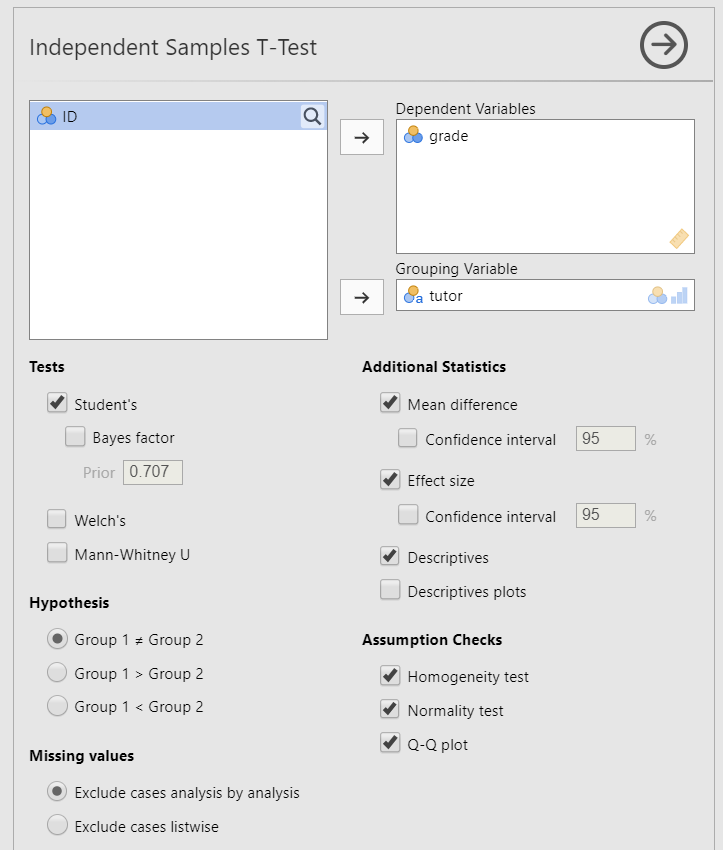
\includegraphics[width=0.8\linewidth]{images/02-independent_t-test/independent_t-test_setup} 

}

\caption{Independent t-test setup in jamovi}\label{fig:unnamed-chunk-2}
\end{figure}

\hypertarget{checking-assumptions-in-jamovi}{%
\section{Checking assumptions in jamovi}\label{checking-assumptions-in-jamovi}}

\hypertarget{testing-normality}{%
\subsection{Testing normality}\label{testing-normality}}

We test for normality using the Shapiro-Wilk test and the Q-Q plot. The Shapiro-Wilk test was not statistically significant (W = .98, \emph{p} = .827); therefore, this indicates the data is normally distributed. Furthermore, the lines are fairly close to the diagonal line in the Q-Q plot. We can conclude that we satisfy the assumption of normality.

\begin{figure}

{\centering 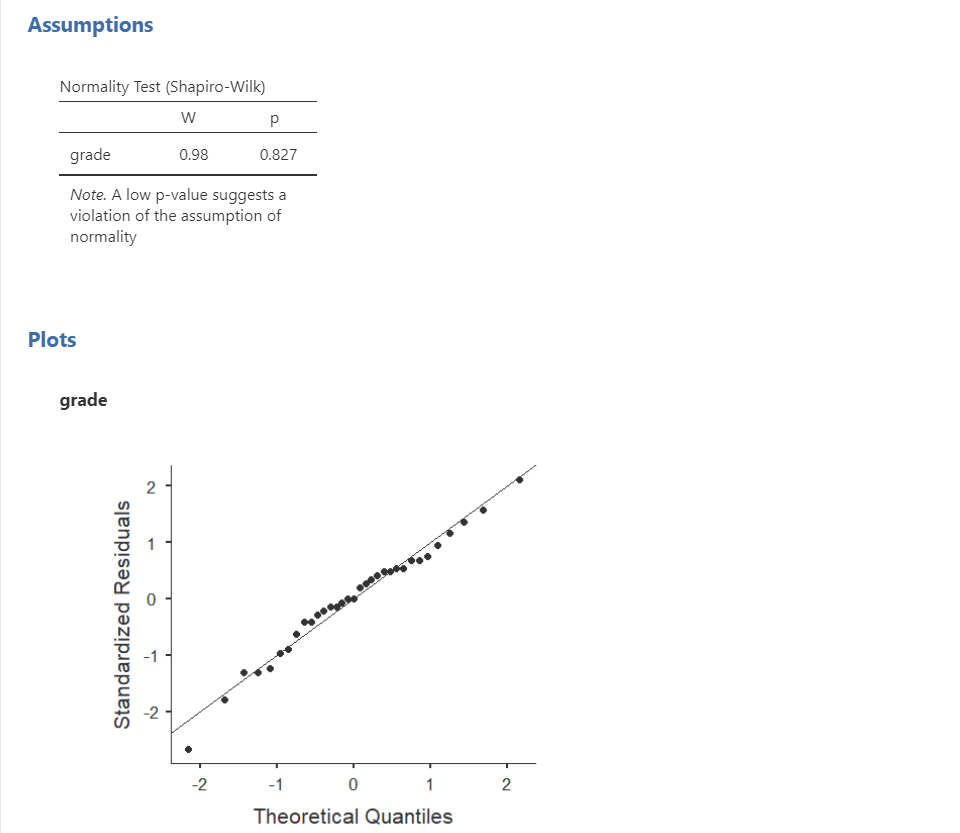
\includegraphics[width=1\linewidth]{images/02-independent_t-test/independent_t-test_normality} 

}

\caption{Testing normality in jamovi}\label{fig:unnamed-chunk-3}
\end{figure}

Remember that we also test for normality by \textbf{looking at our data} (e.g., a histogram) and by examining \textbf{skew and kurtosis}. However, you will need to view them using Exploration --\textgreater{} Descriptives, not in the t-tests menu.

\hypertarget{testing-homogeneity-of-variance}{%
\subsection{Testing homogeneity of variance}\label{testing-homogeneity-of-variance}}

We test for homogeneity of variance using the Levene's test. The Levene's test was not statistically significant (\emph{F} {[}1, 31{]} = 2.49, \emph{p} = .125); therefore, this indicates our data satisfies the assumption of homogeneity of variance. However, I would add a caveat that we have a small sample of data (\emph{n} = 15 for Anastasia and \emph{n} = 18 for Bernadette) and the standard deviations are quite different from one another (SD = 9.00 vs 5.77, respectively). We should have tried to collect more data.

\begin{figure}

{\centering 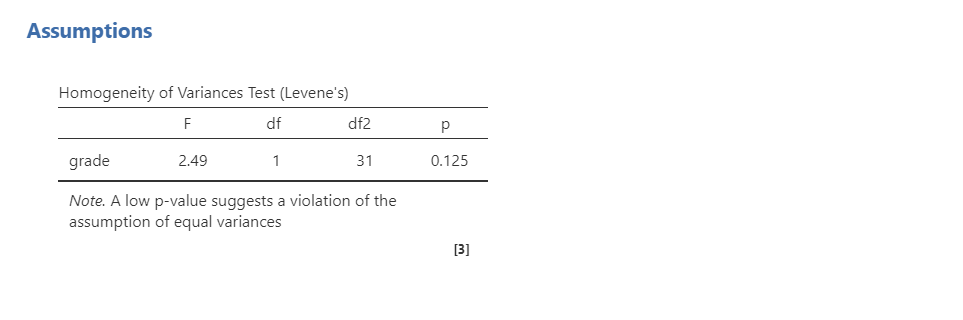
\includegraphics[width=1\linewidth]{images/02-independent_t-test/independent_t-test_homogeneity} 

}

\caption{Testing homogeneity of variance in jamovi}\label{fig:unnamed-chunk-4}
\end{figure}

\hypertarget{interpreting-results}{%
\section{Interpreting results}\label{interpreting-results}}

Once we are satisfied we have satisfied the assumptions for the independent t-test, we can interpret our results.

\begin{figure}

{\centering 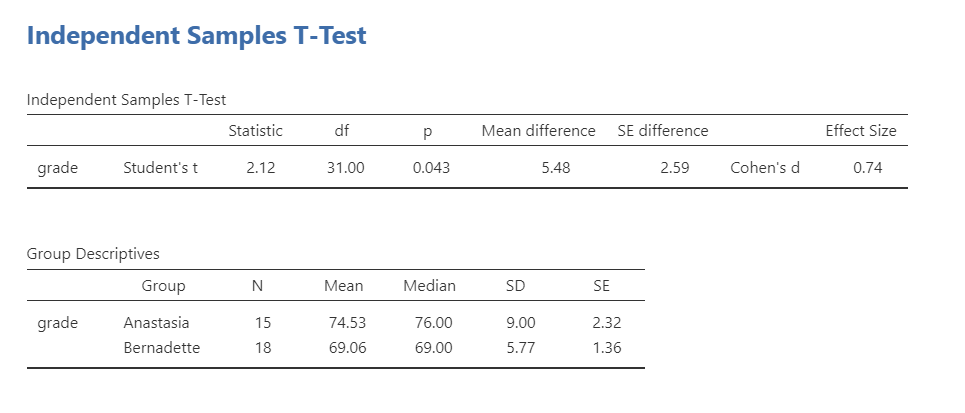
\includegraphics[width=1\linewidth]{images/02-independent_t-test/independent_t-test_ind-results} 

}

\caption{Independent t-test results in jamovi}\label{fig:unnamed-chunk-5}
\end{figure}

Our p-value is less than .05, so our results are statistically significant. We can write up our results in APA something like this:

\begin{quote}
Anastasia's students (\emph{M} = 74.53, \emph{SD} = 9.00, \emph{n} = 15) had significantly higher grades than Bernadette's students (\emph{M} = 69.06, \emph{SD} = 5.77, \emph{n}~= 18), \emph{t} (31) = 2.12, \emph{p} = .043, \emph{d} = .74.
\end{quote}

Sometimes, people like to put the statistics inside a parentheses. In that case, you need to change the parentheses around the degrees of freedom as brackets. Here's another example write-up of the results in APA style:

\begin{quote}
I tested the difference in grades between Anastasia's students (\emph{M} = 74.53, \emph{SD} = 9.00, \emph{n} = 15) and Bernadette's students (\emph{M} = 69.06, \emph{SD} = 5.77, \emph{n}~= 18). An independent samples t-test showed that the 5.48 mean difference between the tutor's student was statistically significant (\emph{t} {[}31{]} = 2.12, \emph{p} = .043, \emph{d} = .74).
\end{quote}

\hypertarget{additional-information-about-the-independent-t-test}{%
\section{Additional information about the independent t-test}\label{additional-information-about-the-independent-t-test}}

\hypertarget{positive-and-negative-t-values}{%
\subsection{Positive and negative t values}\label{positive-and-negative-t-values}}

Students often worry about positive or negative t-statistic values and are unsure how to interpret it. Positive or negative t-statistic values simply occur based on which group is listed first. Our t-statistic above is positive because we tested the difference between Anastasia and Bernadette: (Anastasia - Bernadette) = (74.53 - 69.06) = (5.48).

However, if we flipped it and tested the difference between Bernadette and Anastasia, our mean difference would be -5.48 and our t-statistic would be -2.12.

All that is to say, \emph{your positive or negative t-statistic is arbitrary}. So do not fret!

However, it is important the sign of your t-statistic matches what you report. For example, notice the difference:

\begin{quote}
\begin{enumerate}
\def\labelenumi{\arabic{enumi}.}
\tightlist
\item
  Anastasia's students had \textbf{higher} grades than Bernadette's, \emph{t} (31) = \textbf{2.12}, \emph{p} = .043, \emph{d} = .74.
\item
  Bernadette's students had \textbf{lower} grades than Anastasia's, \emph{t} (31) = \textbf{-2.12}, \emph{p} = .043, \emph{d} = .74.
\end{enumerate}
\end{quote}

One last note: this positive or negative t-statistic is only relevant for the independent and dependent t-test. You will not get negative values for the F-statistic or chi-square tests!

\hypertarget{what-if-i-violated-assumptions}{%
\subsection{What if I violated assumptions?}\label{what-if-i-violated-assumptions}}

The great news is that jamovi includes the Welch's t-statistic and the non-parametric version of the independent t-test (Mann-Whitney U)!

The Welch's t-test has three main differences from the independent samples t-test: (a) the standard error (SE) is not a pooled estimate, (b) the degrees of freedom are calculated very different (not \emph{N} - 2), and (c) it does not have an assumption of homogeneity of variance. Note that Welch's t-test is not a non-parametric test because it still has the assumption of a normal distribution.

The Mann-Whitney U is not calculated based on the mean but rather the median and compares ranks of values across the two groups: it has no assumptions about the distribution of data or homogeneity of variances.

Here's what statistic you should choose based on satisfying assumptions:

\begin{longtable}[]{@{}lll@{}}
\toprule
\begin{minipage}[b]{0.39\columnwidth}\raggedright
\strut
\end{minipage} & \begin{minipage}[b]{0.25\columnwidth}\raggedright
\textbf{Normality: satisfied}\strut
\end{minipage} & \begin{minipage}[b]{0.27\columnwidth}\raggedright
\textbf{Normality: not satisfied}\strut
\end{minipage}\tabularnewline
\midrule
\endhead
\begin{minipage}[t]{0.39\columnwidth}\raggedright
\textbf{Homogeneity of Variance: satisfied}\strut
\end{minipage} & \begin{minipage}[t]{0.25\columnwidth}\raggedright
independent samples t-test\strut
\end{minipage} & \begin{minipage}[t]{0.27\columnwidth}\raggedright
Mann-Whitney U\strut
\end{minipage}\tabularnewline
\begin{minipage}[t]{0.39\columnwidth}\raggedright
\textbf{Homogeneity of Variance: not satisfied}\strut
\end{minipage} & \begin{minipage}[t]{0.25\columnwidth}\raggedright
Welch's t-test\strut
\end{minipage} & \begin{minipage}[t]{0.27\columnwidth}\raggedright
Mann-Whitney U\strut
\end{minipage}\tabularnewline
\bottomrule
\end{longtable}

Here is what the output for all three tests look like:

\begin{figure}

{\centering 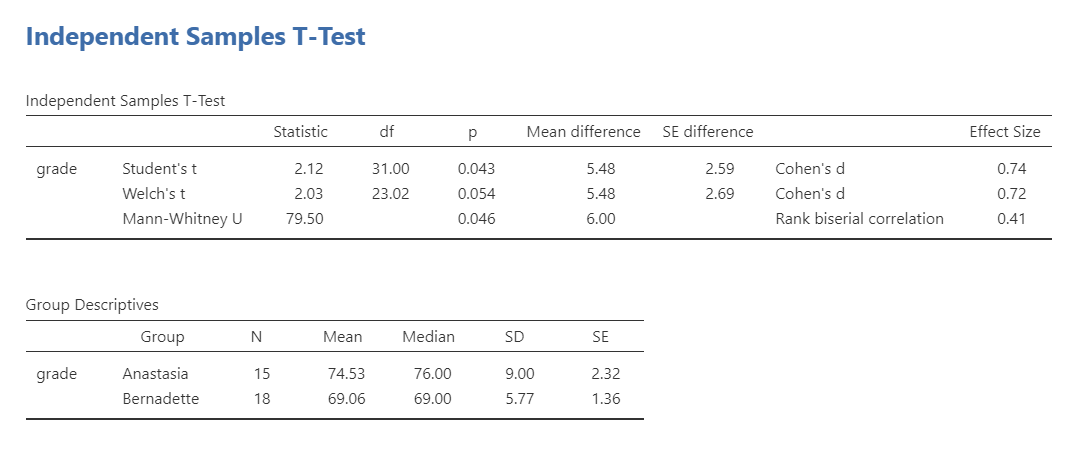
\includegraphics[width=1\linewidth]{images/02-independent_t-test/independent_t-test_full-results} 

}

\caption{All independent t-test results in jamovi}\label{fig:unnamed-chunk-6}
\end{figure}

\hypertarget{welchs-t-test-in-jamovi}{%
\subsubsection{Welch's t-test in jamovi}\label{welchs-t-test-in-jamovi}}

To conduct this in jamovi, under Tests select \texttt{Welch\textquotesingle{}s}. You will interpret the results similarly to the independent t-test:

\begin{quote}
Using a Welch's t-test, there was not a statistically significant difference in grades between Anastasia's students (\emph{M} = 74.53, \emph{SD} = 9.00, \emph{n} = 15) and Bernadette's students (\emph{M} = 69.06, \emph{SD} = 5.77, \emph{n} = 18), \emph{t} (23.02) = 2.03, \emph{p} = .054, \emph{d} = .72.
\end{quote}

Why is it no longer statistically significant? Which result should you trust? In reality, the difference in \emph{p}-values is likely due to chance. However, the independent t-test and Welch's test have different strengths and weaknesses. If the two populations really do have equal variances, then the independent t-test is slightly more powerful (lower Type II error rate) than the Welch's test. However, if they \emph{don't} have the same variances, then the assumptions of the independent t-test are violated and you may not be able to trust the results; you may end up with a higher Type I error rate. So it's a trade-off.

Which should you use? I tend to prefer always using Welch's t-test because if the variances are equal, then there will be practically no difference between the independent and Welch's t-test. But if the variances are not equal, then Welch's t-test will outperform the independent t-test. For that reason, defaulting to the Welch's t-test makes most sense to me.

\hypertarget{mann-whitney-u-test}{%
\subsubsection{Mann-Whitney U test}\label{mann-whitney-u-test}}

If you do not satisfy the assumption of normality (regardless of whether you satisfy the assumption of homogeneity of variance), you should either try to transform your data to be normally distributed or you will need to use a non-parametric test. In this case, if you originally wanted to perform an independent t-test, the non-parametric equivalent test is the Mann-Whitney U test.

I will not go into specifics, but the idea behind the Mann-Whitney U test is that you take all the values (regardless of group) and rank them. You then sum the ranks across groups and calculate your U statistic and p-value. You interpret the p-value like you normally would, but there are differences in how we report the results because this statistic is based on the \emph{median} not the \emph{mean}.

\begin{quote}
Using the Mann-Whitney U test, there was a statistically significant difference in grades between Anastasia's students (\emph{Mdn} = 76, \emph{n} = 15) and Bernadette's students (\emph{Mdn} = 69, \emph{n}~= 18), \emph{t} (23.02) = 2.03, \emph{p} = .054, \emph{d} = .72.
\end{quote}

\hypertarget{your-turn}{%
\section{Your turn!}\label{your-turn}}

Open the \texttt{Sample\_Dataset\_2014.xlsx} file that we will be using for all Your Turn exercises.

Perform independent t-tests based on the following research questions. Think critically about whether you should be using a one-tailed or two-tailed hypothesis and check your assumptions so you know which test to use!

To get the most out of these exercises, try to first find out the answer on your own and then use the drop-down menus to check your answer.

\begin{enumerate}
\def\labelenumi{\arabic{enumi}.}
\item
  \textbf{Does height differ by gender (Gender: male = 0, female = 1)?}

  \begin{itemize}
  \item
    Should you use a one-tailed or two-tailed hypothesis? one-tailed two-tailed
  \item
    Which statistic should you use based on your assumptions? independent t-test Welch's t-test Mann Whitney U
  \item
    Does height differ by gender? yes no
  \end{itemize}
\item
  \textbf{Do athletes (Athlete: athletes = 1, non-athlete = 0) have faster sprint times than non-athletes?}

  \begin{itemize}
  \item
    Should you use a one-tailed or two-tailed hypothesis? one-tailed two-tailed
  \item
    Which statistic should you use based on your assumptions? independent t-test Welch's t-test Mann Whitney U
  \item
    Do athletes have faster sprint times than non-athletes? yes no
  \end{itemize}
\item
  \textbf{Do students who live on campus (LiveOnCampus: on campus = 1, off campus = 0) have higher English scores than students who live off campus?}

  \begin{itemize}
  \item
    Should you use a one-tailed or two-tailed hypothesis? one-tailed two-tailed
  \item
    Which statistic should you use based on your assumptions? independent t-test Welch's t-test Mann Whitney U
  \item
    Does students who live on campus have higher English scores? yes no
  \end{itemize}
\item
  \textbf{Does athletic status relate to math scores?}

  \begin{itemize}
  \item
    Should you use a one-tailed or two-tailed hypothesis? one-tailed two-tailed
  \item
    Which statistic should you use based on your assumptions? independent t-test Welch's t-test Mann Whitney U
  \item
    Does athletic status relate to math scores? yes no
  \end{itemize}
\end{enumerate}

\hypertarget{dependent-t-test}{%
\chapter{Dependent t-test}\label{dependent-t-test}}

\hypertarget{what-is-the-dependent-t-test}{%
\section{What is the dependent t-test?}\label{what-is-the-dependent-t-test}}

The dependent t-test is used to test the difference in our dependent variable between two categories in which participants are the \emph{same} across categories. Our category variable is our independent variable. In other words, we use the independent t-test when we have a research question with a \textbf{continuous dependent variable} and a \textbf{categorical independent variable with two categories in which the same participants are in each category}.

The dependent t-test is also called a dependent samples t-test or paired samples t-test.

\hypertarget{data-set-up-1}{%
\section{Data set-up}\label{data-set-up-1}}

To conduct the dependent t-test, we first need to ensure our data is set-up properly in our dataset. This requires having two columns: one is our dependent variable score for the participant in one category and the other column is our dependent variable score for the participant in the other category. Each row is a unique participant or unit of analysis. Here's what example data may look like if we were testing for differences in test scores across the same participants in the fall and spring:

\begin{longtable}[]{@{}llr@{}}
\caption{Example data for the dependent t-test}\tabularnewline
\toprule
ID & TestScore\_Fall & TestScore\_Spring\tabularnewline
\midrule
\endfirsthead
\toprule
ID & TestScore\_Fall & TestScore\_Spring\tabularnewline
\midrule
\endhead
1 & 75 & 86\tabularnewline
2 & 79 & 80\tabularnewline
3 & 65 & 75\tabularnewline
4 & 81 & 79\tabularnewline
5 & 73 & 82\tabularnewline
6 & 72 & 84\tabularnewline
7 & 69 & 90\tabularnewline
8 & 60 & 72\tabularnewline
9 & 75 & 75\tabularnewline
10 & 74 & 81\tabularnewline
\bottomrule
\end{longtable}

In the example data above, what is your \textbf{independent variable}? ID Semester TestScore

In the example data above, what is your \textbf{dependent variable}? ID Semester Test Score

\hypertarget{the-math-behind-the-independent-t-test-1}{%
\section{The math behind the independent t-test}\label{the-math-behind-the-independent-t-test-1}}

The basic math of the dependent t-test is the mean difference divided by the standard error, which is estimated based on the standard deviation and sample size (N).

\(t = \frac{\bar{X}_1 - \bar{X}_2}{s_d/ \sqrt{N}}\)

\hypertarget{assumptions-1}{%
\section{Assumptions}\label{assumptions-1}}

As a parametric test, the independent t-test has the same assumptions as other parametric tests minus the homogeneity of variance assumption because we are dealing with the same people across categories

\begin{enumerate}
\def\labelenumi{\arabic{enumi}.}
\item
  The \emph{differences in scores} in the dependent variable are \textbf{normally distributed}
\item
  The dependent variable is \textbf{interval or ratio} (i.e., continuous)
\item
  Scores are \textbf{independent} across participants
\end{enumerate}

We cannot \underline{test} the second and third assumptions; rather, those are based on knowing your data.

However, we can and should test for the first assumption. Fortunately, the dependent samples t-test in jamovi has two check boxes under ``Assumption Checks'' that lets us test normality.

\hypertarget{in-jamovi}{%
\section{In jamovi}\label{in-jamovi}}

Let's run an example with data from lsj-data. Open data from your Data Library in ``lsj-data''. Select and open ``Chico''. This dataset is hypothetical data from Dr.~Chico's class in which students took two tests: one early in the semester and one later in the semester. Dr.~Chico thinks that the first test is a ``wake up call'' for students. When they realise how hard her class really is, they'll work harder for the second test and get a better mark. Is she right? Let's test it!

\begin{enumerate}
\def\labelenumi{\arabic{enumi}.}
\item
  To perform an dependent t-test in jamovi, go to the Analyses tab, click the T-Tests button, and choose ``Paired Samples T-Test''.
\item
  Move both measurements of your dependent variable (\texttt{grade\_test1} and \texttt{grade\_test2}) to the Paired Variables box.
\item
  Under Tests, select \texttt{Student\textquotesingle{}s}
\item
  Under Hypothesis, choose the correct hypothesis: Measure 1 is not equal to Measure 2 Measure 1 \textgreater{} Measure 2 Measure 1 \textless{} Measure 2
\item
  Under Additional Statistics, select \texttt{Mean\ difference}, \texttt{Effect\ size}, and \texttt{Descriptives}.
\item
  Under Assumption Checks, select both options: \texttt{Normality\ test} and \texttt{Q-Q\ plot}.
\end{enumerate}

When you are done, your setup should look like this

\begin{figure}

{\centering 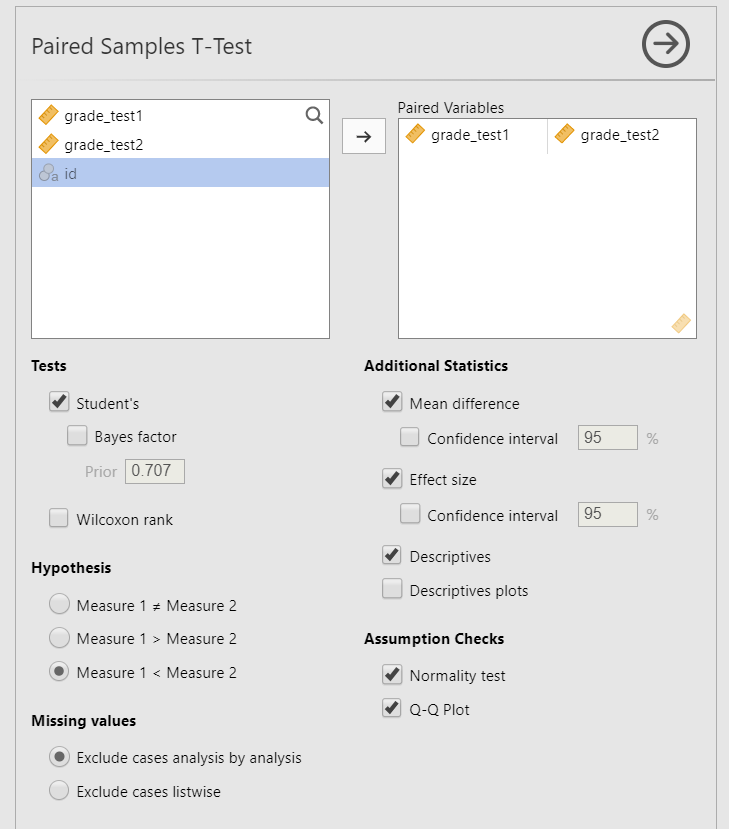
\includegraphics[width=0.8\linewidth]{images/03_dependent_t-test/dependent_setup} 

}

\caption{Dependent t-test setup in jamovi}\label{fig:unnamed-chunk-1}
\end{figure}

\hypertarget{checking-assumptions-in-jamovi-1}{%
\subsection{Checking assumptions in jamovi}\label{checking-assumptions-in-jamovi-1}}

\hypertarget{testing-normality-1}{%
\subsubsection{Testing normality}\label{testing-normality-1}}

We test for normality using the Shapiro-Wilk test and the Q-Q plot. The Shapiro-Wilk test was not statistically significant (W = .97, \emph{p} = .678); therefore, this indicates the data is normally distributed. Furthermore, the lines are fairly close to the diagonal line in the Q-Q plot (although it's a bit hard to tell because our sample size is small). We can conclude that we satisfy the assumption of normality.

\begin{figure}

{\centering 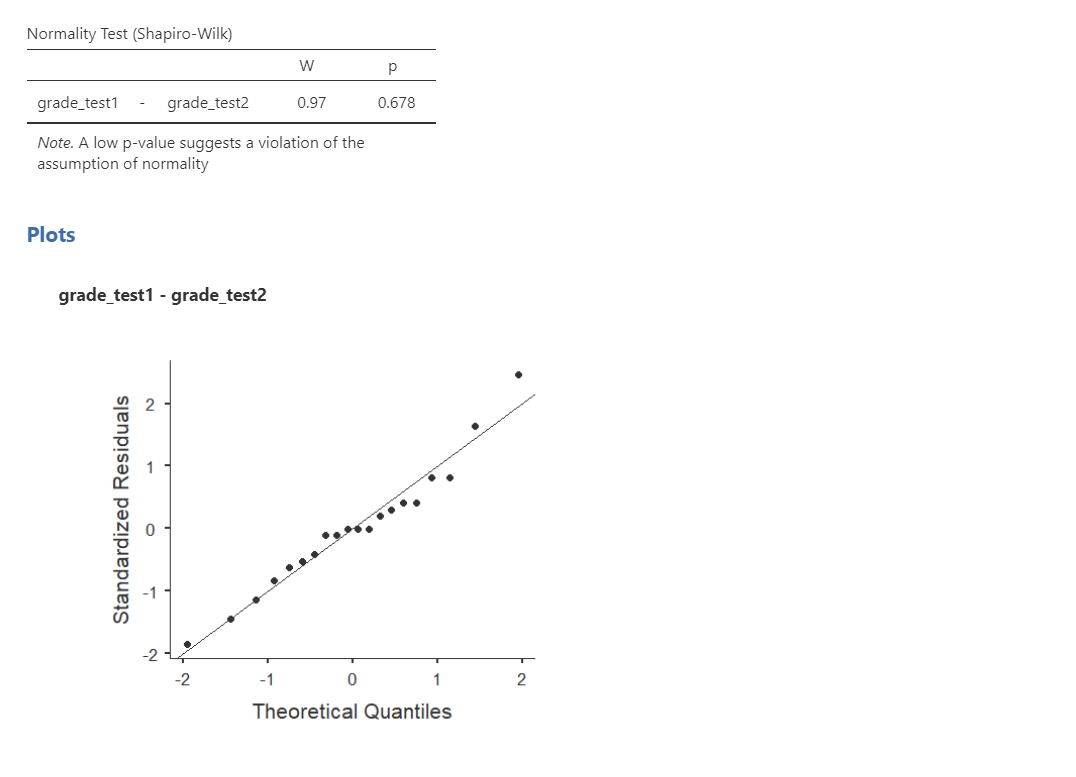
\includegraphics[width=1\linewidth]{images/03_dependent_t-test/dependent_normality} 

}

\caption{Testing normality in jamovi}\label{fig:unnamed-chunk-2}
\end{figure}

\hypertarget{interpreting-results-1}{%
\subsection{Interpreting results}\label{interpreting-results-1}}

Once we are satisfied we have satisfied the assumptions for the dependent t-test, we can interpret our results.

\begin{figure}

{\centering 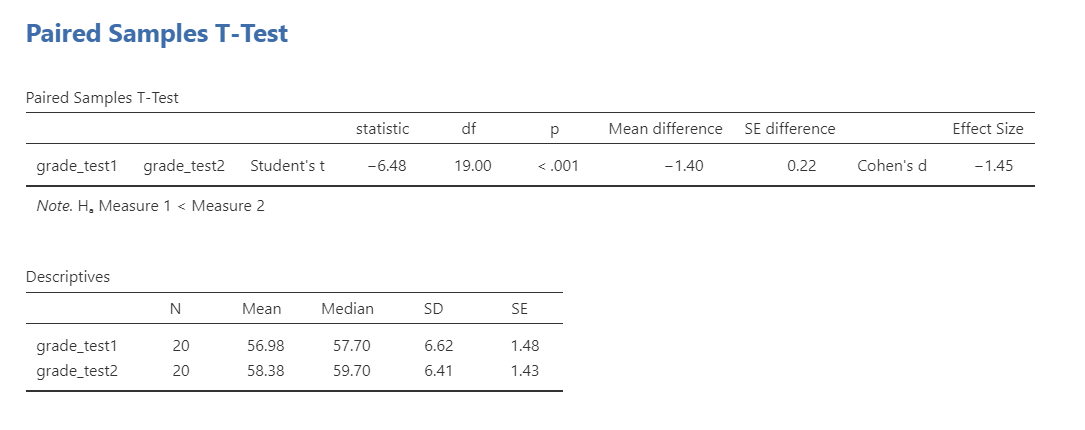
\includegraphics[width=1\linewidth]{images/03_dependent_t-test/dependent_results} 

}

\caption{Dependent t-test results in jamovi}\label{fig:unnamed-chunk-3}
\end{figure}

Our p-value is less than .05, so our results are statistically significant. We can write up our results in APA something like this:

\begin{quote}
The 20 students in Dr.~Chico's class performed worse on the first test (\emph{M} = 56.98, \emph{SD} = 6.62) than they did on the second test (\emph{M} = 58.38, \emph{SD} = 6.41), \emph{t}(19) = -6.48, \emph{p} \textless{} .001, \emph{d} = -1.45.
\end{quote}

Remember in the previous chapter that our t-test can be negative but we can always flip the interpretation. Here's another example of how we could write-up our results in APA style:

\begin{quote}
Dr.~Chico's hypothesis was correct in that her 20 students performed better on the second test (\emph{M} = 58.38, \emph{SD} = 6.41) than they did on the first test (\emph{M} = 56.98, \emph{SD} = 6.62), \emph{t}(19) = 6.48, \emph{p} \textless{} .001, \emph{d} = 1.45.
\end{quote}

\hypertarget{what-if-i-violated-assumptions-1}{%
\section{What if I violated assumptions?}\label{what-if-i-violated-assumptions-1}}

If you violated the assumption of normality and no transformation fixed your data, then you can perform the non-parametric version of the dependent t-test called the Wilcoxon Rank test. As a reminder, non-parametric tests do not make assumptions about the distribution of data because it deals with the \emph{median} not the \emph{mean}.

Here is the output for both the dependent t-test and the Wilcoxon rank test:

\begin{figure}

{\centering 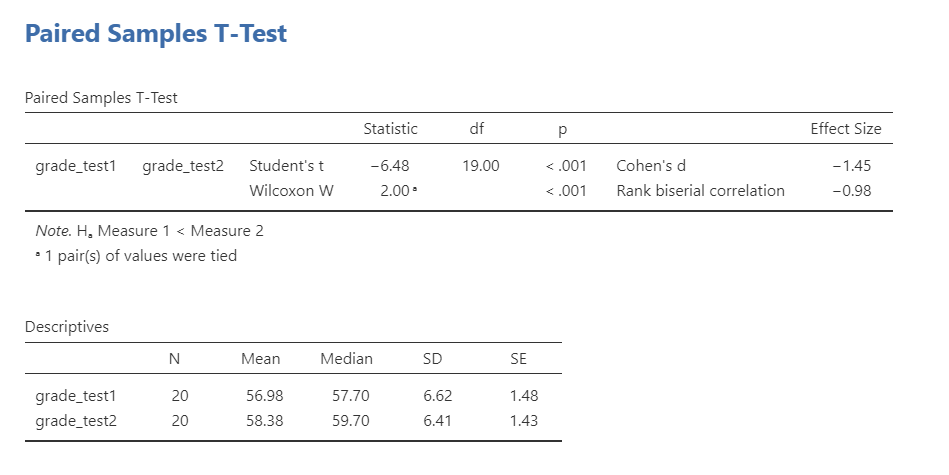
\includegraphics[width=1\linewidth]{images/03_dependent_t-test/dependent_results_full} 

}

\caption{All independent t-test results in jamovi}\label{fig:unnamed-chunk-4}
\end{figure}

\hypertarget{wilcoxon-rank-in-jamovi}{%
\subsubsection{Wilcoxon rank in jamovi}\label{wilcoxon-rank-in-jamovi}}

To conduct this in jamovi, under Tests select \texttt{Wilcoxon\ rank}. You will interpret the results similarly to the dependent t-test:

\begin{quote}
Using Wilcoxon rank test, students' test scores were significantly higher at the second test (\emph{Mdn} = 59.70) than at the first test (\emph{Mdn} = 57.70), W = 2.00, \emph{p} \textless{} .001.
\end{quote}

The note about tied values is not necessary to discuss. It is just telling us one participant had identical values for both test1 and test2 (student15).

\hypertarget{your-turn-1}{%
\section{Your turn!}\label{your-turn-1}}

Open the \texttt{Sample\_Dataset\_2014.xlsx} file that we use for all Your Turn exercises.

Perform dependent t-tests based on the following research questions. Think critically about whether you should be using a one-tailed or two-tailed hypothesis and check your assumptions so you know which test to use!

To get the most out of these exercises, try to first find out the answer on your own and then use the drop-down menus to check your answer.

\textbf{Note}: Technically, none of our data is suitable for a dependent t-test in this dataset. We will pretend that the four test score variables (\texttt{English}, \texttt{Reading}, \texttt{Math}, and \texttt{Writing}) are really four measurements of the same underlying test. In reality, we would analyze this data using correlation.

\begin{enumerate}
\def\labelenumi{\arabic{enumi}.}
\item
  \textbf{Do students perform better on the English test than they do the Writing test?}

  \begin{itemize}
  \item
    Should you use a one-tailed or two-tailed hypothesis? one-tailed two-tailed
  \item
    Which statistic should you use based on your assumptions? dependent t-test Wilcoxon rank
  \item
    Do students perform better on the English test than they do the Writing test? yes no
  \end{itemize}
\item
  \textbf{Does students' English scores relate to their Reading scores?}

  \begin{itemize}
  \item
    Should you use a one-tailed or two-tailed hypothesis? one-tailed two-tailed
  \item
    Which statistic should you use based on your assumptions? dependent t-test Wilcoxon rank
  \item
    Does students' English scores relate to their Reading scores? yes no
  \end{itemize}
\end{enumerate}

\hypertarget{part-anova}{%
\part{ANOVA}\label{part-anova}}

\hypertarget{one-way-anova}{%
\chapter{One-way ANOVA}\label{one-way-anova}}

\hypertarget{what-is-the-one-way-anova}{%
\section{What is the one-way ANOVA?}\label{what-is-the-one-way-anova}}

The one-way analysis of variance (ANOVA) is used to test the difference in our dependent variable between \underline{three or more} different groups of observations. Our grouping variable is our independent variable. In other words, we use the one-way ANOVA when we have a research question with a \textbf{continuous dependent variable} and a \textbf{categorical independent variable with three or more categories in which different participants are in each category}.

The one-way ANOVA is also known as an independent factor ANOVA.

One thing to keep in mind is the one-way ANOVA is an omnibus statistic that tests against the null hypothesis that the three or more means are the same. It does not tell us where the mean differences are (e.g., that 1 \textgreater{} 2); for that, we need planned contrasts or post-hoc procedures, which you'll learn about later. Therefore, the null and alternative hypotheses for the one-way ANOVA are as follows:

\begin{itemize}
\tightlist
\item
  \(H_0\): There is \textbf{no difference} in means between the groups. In other words, the means for the three or more groups are the \textbf{same}.
\item
  \(H_1\): There is \textbf{a difference} in means between the groups. In other words, the means for the three or more groups are \textbf{different}.
\end{itemize}

\hypertarget{data-set-up-2}{%
\section{Data set-up}\label{data-set-up-2}}

To conduct the one-way ANOVA, we first need to ensure our data is set-up properly in our dataset. This requires having two columns: one with our continuous dependent variable and one indicating which group the participant is in. Each row is a unique participant or unit of analysis. Here's what example data may look like if we were testing for differences in a test score by students in my fall, spring, or summer semesters of my course

\begin{longtable}[]{@{}llr@{}}
\caption{Example data for the one-way ANOVA}\tabularnewline
\toprule
ID & Semester & TestScore\tabularnewline
\midrule
\endfirsthead
\toprule
ID & Semester & TestScore\tabularnewline
\midrule
\endhead
1 & Fall & 86\tabularnewline
2 & Fall & 80\tabularnewline
3 & Fall & 75\tabularnewline
4 & Spring & 79\tabularnewline
5 & Spring & 82\tabularnewline
6 & Spring & 84\tabularnewline
7 & Summer & 90\tabularnewline
8 & Summer & 72\tabularnewline
9 & Summer & 75\tabularnewline
\bottomrule
\end{longtable}

In the example data above, what is your \textbf{independent variable}? ID Semester TestScore

In the example data above, what is your \textbf{dependent variable}? ID Semester TestScore

\hypertarget{why-not-multiple-t-tests}{%
\section{Why not multiple t-tests?}\label{why-not-multiple-t-tests}}

In the example above, we have three groups: fall, spring, and summer. We could just perform three separate t-tests: fall vs.~spring, fall vs.~summer, and spring vs.~summer.

However, the reason we do not perform multiple t-tests is to reduce our Type I error rate. If I had performed three separate t-tests, set my alpha (Type I error rate) at 5\%, and knew for a fact the effects do not actually exist, then each test has a probability of a Type I error rate of 5\%. Because we are running three tests, our alpha rate actually becomes 1 - (.95\textsuperscript{3})= 1 - .857 = 14.3\%! So now our \emph{familywise} or \emph{experimentwise}~error rate is 14.3\%, not the 5\% we originally set alpha at.

With three groups, that's not so bad, but let's see what happens with more tests we perform:

\begin{itemize}
\tightlist
\item
  \textbf{1 test}: 1 - (.95\textsuperscript{1})= 1 - .95 = \textbf{5\%}
\item
  \textbf{2 tests}: 1 - (.95\textsuperscript{2})= 1 - .9025 = \textbf{9.8\%}
\item
  \textbf{3 tests}: 1 - (.95\textsuperscript{3})= 1 - .857 = \textbf{14.3\%}
\item
  \textbf{4 tests}: 1 - (.95\textsuperscript{4})= 1 - .814 = \textbf{18.6\%}
\item
  \textbf{5 tests}: 1 - (.95\textsuperscript{5})= 1 - .774 = \textbf{22.6\%}
\item
  \textbf{10 tests}: 1 - (.95\textsuperscript{10})= 1 - .598 = \textbf{40.1\%}
\item
  \textbf{20 tests}: 1 - (.95\textsuperscript{20})= 1 - .358 = \textbf{64.1\%}
\end{itemize}

Ouch! 10 tests would have a Type I error rate of 40\%! That means that if we performed 10 statistical tests (assuming the effect does not exist), then 40\% of the results would be statistically significant by chance alone and would be a false positive. That's not good!

Therefore, we use the one-way ANOVA as one test to see if there is a difference overall. We can also do things to control or limit our familywise error rate, which I'll get into later.

\hypertarget{the-math-behind-the-one-way-anova}{%
\section{The math behind the one-way ANOVA}\label{the-math-behind-the-one-way-anova}}

The basic math of the one-way ANOVA is the between-group variance (mean squares - between groups) divided by the within-group variance (mean squares - within groups).

\(F = \frac{BG \:variance}{WG \:variance} = \frac{MS_{BG}}{MS_{WG}} = \frac{\frac{SS_{BG}}{df_{BG}}}{\frac{SS_{WG}}{df_{WG}}}\)

There are specific formulas for the between-group (also called the model) sum of squares (SS) and within-group (also called the residual) sum of squares. Keep in mind the following symbols:

\begin{itemize}
\tightlist
\item
  n/N = sample size (little n is per group, big N is the overall sample)
\item
  k = number of groups
\item
  X = mean
\item
  s = standard deviation
\end{itemize}

The between-group SS is the \emph{variation between group means}. The calculations you see below is to subtract the overall mean (\(\bar{X}_{grand}\)) from the group mean (\(\bar{X_k}\)), square that mean difference, multiply that by the sample size in that group (\(n_k\)), and then sum all the results of doing that per group.

\(SS_{BG} = \sum{n_k}(\bar{X_k}-\bar{X}_{grand})^2\)

\(df_{BG} = k - 1\)

The within-group SS is the \emph{variation of scores within groups}. The calculations you see below is to take the sample size in that group (\(n_k\)) and subtract 1 from it, then multiply it by the group's variance (\(s_k^2\), which is standard deviation squared), and then sum all the results of doing that per group.

\(SS_{WG} = \sum{s_k^2}(n_k - 1)\)

\(df_{WG} = N - k\)

In other words, the F-ratio is a ratio of the group or experimental effect by the individual differences in performance.

For our F-ratio to be statistically significant, we want to \emph{maximize} the variance between groups (numerator) and \emph{minimize} the variance within groups (denominator). This is depicted in the image below. On the left (a) the arrows show the differences in the group means. On the right (b) the arrows highlight the variability within each group. You want to maximize (a) and minimize (b).

\begin{figure}

{\centering 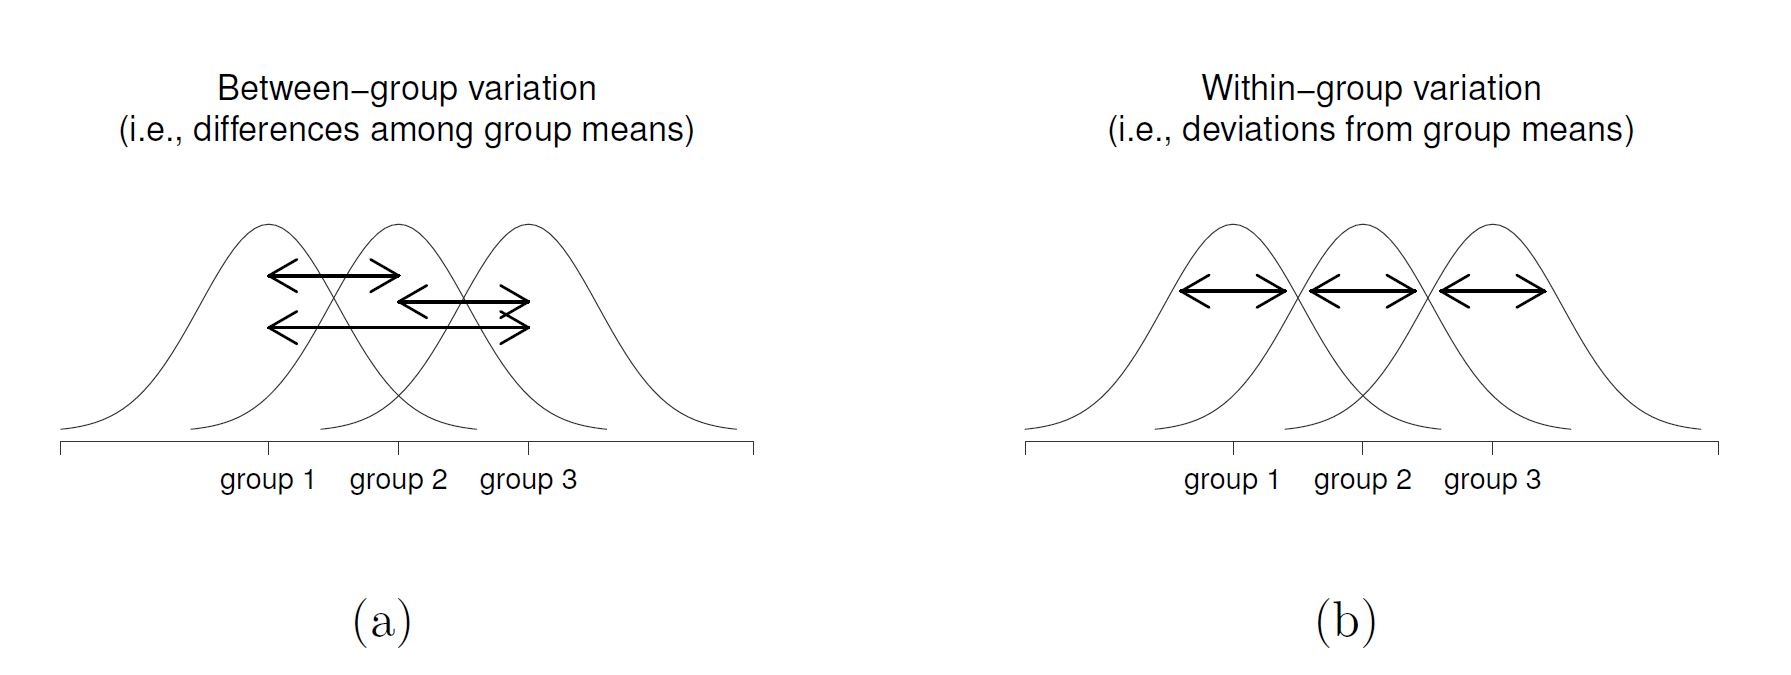
\includegraphics[width=0.8\linewidth]{images/04_one-way-anova/anova graphic} 

}

\caption{Graphical illustration of the one-way ANOVA}\label{fig:unnamed-chunk-1}
\end{figure}

\hypertarget{an-example-with-the-math}{%
\subsection{An example with the math}\label{an-example-with-the-math}}

In case it's useful, read below. If your eyes are glazing over, just move to the next section.

You can read the example dataset below. I've pulled the relevant data here so we can go through a hand calculation ourselves.

\begin{longtable}[]{@{}llll@{}}
\toprule
Drug & N & Mean & Variance\tabularnewline
\midrule
\endhead
Anxifree & 6 & 0.7167 & .1537\tabularnewline
Joyzepam & 6 & 1.4833 & .0457\tabularnewline
Placebo & 6 & 0.4500 & .0790\tabularnewline
\textbf{Overall} & \textbf{18} & \textbf{0.8833} & \textbf{.28}\tabularnewline
\bottomrule
\end{longtable}

Let's start with the easy stuff! Let's calculate our degrees of freedom.

\(df_{BG} = k - 1 = 3 -1 = 2\)

\(df_{WG} = N - k = 18 - 3 = 15\)

Now let's move to the more complicated ones.

\(\begin{aligned} SS_{BG} &= \sum{n_k}(\bar{X_k}-\bar{X}_{grand})^2 \\ SS_{BG} &= 6(.7167-.8833)^2 + 6(1.4833-.8833)^2 + 6(.4500-.8833)^2 \\ SS_{BG} &= 6(-.1666)^2 + 6(.6)^2 + 6(-.4333)^2 \\ SS_{BG} &= 6(.0278) + 6(.36) + 6(.1877) \\ SS_{BG} &= .1665 + 2.16 + 1.1262 \\ SS_{BG} &= 3.453 \end{aligned}\)

Then we can calculate our \(MS_{BG}\).

\(MS_{BG} = \frac{SS_{BG}}{df_{BG}} = \frac{3.453}{2} = 1.727\)

Let's move to our \(SS_{WG}\).

\(\begin{aligned} SS_{WG} &= \sum{s_k^2}(n_k - 1) \\ SS_{WG} &= .1537(6-1) + .0457(6-1) + .0790(6-1) \\ SS_{WG} &= .1537(5) + .0457(5) + .0790(5) \\ SS_{WG} &= .7685 + .2285 + .3950 \\ SS_{WG} &= 1.392 \end{aligned}\)

Now we can calculate our \(MS_{WG}\).

\(MS_{WG} = \frac{SS_{WG}}{df_{WG}} = \frac{1.392}{15} = .0928\)

Now all that's left is to calculate \(F\)!

\(F = \frac{MS_{BG}}{MS_{WG}} = \frac{1.726}{.0928} = 18.60\)

Compare to the \(F\), \(df_{WG}\), and \(df_{BG}\) in the output below in jamovi! Notice how close we are. Also notice how many decimals I retained throughout the analyses. I was a bit off when I first did this with only two decimals throughout. Retaining four decimals throughout got me only \textasciitilde one-hundredth of a decimal off from the actual results. Neat!

\hypertarget{anova-assumptions}{%
\section{Assumptions}\label{anova-assumptions}}

As a parametric test, the one-way ANOVA has the same assumptions as other parametric tests:

\begin{enumerate}
\def\labelenumi{\arabic{enumi}.}
\item
  The dependent variable is \textbf{normally distributed}
\item
  Variances in the two groups are roughly equal (i.e., \textbf{homogeneity of variances})
\item
  The dependent variable is \textbf{interval or ratio} (i.e., continuous)
\item
  Scores are \textbf{independent} between groups
\end{enumerate}

We cannot \underline{test} the third and fourth assumptions; rather, those are based on knowing your data. However, we can and should test for the first two assumptions. Fortunately, the one-way ANOVA in jamovi has three check boxes under ``Assumption Checks'' that lets us test for both assumptions.

\hypertarget{anova-is-robust-to-violations}{%
\subsection{ANOVA is robust to violations}\label{anova-is-robust-to-violations}}

Although we should meet the assumptions as much as possible, in general the F-statistic is \emph{robust} to violations of normality and homogeneity of variance. This means that you can still run the one-way ANOVA if you violate the assumptions, but \emph{only when group sizes are equal or nearly equal}. If you have vastly different variances (such as 2:1 ratio or greater) or vastly different group sizes (such as a 2:1 ratio or greater), and especially if one group is small (such as 10 or fewer cases), then your F-statistic is likely to be very wrong. For example, if your larger group has the larger variance, then your F-statistic is likely to be non-significant or smaller than it should be; however, if your larger group has smaller variance,then your F-statistic is likely to be significant or bigger than it should be!

\hypertarget{in-jamovi-1}{%
\section{In jamovi}\label{in-jamovi-1}}

Let's run an example with data from lsj-data. Open data from your Data Library in ``lsj-data''. Select and open ``clinicaltrial''. This dataset is hypothetical data of a clinical trial in which you are testing a new antidepressant drug called \emph{Joyzepam}. In order to construct a fair test of the drug's effectiveness, the study involves three separate drugs to be administered. One is a placebo, and the other is an existing antidepressant / anti-anxiety drug called \emph{Anxifree}. A collection of 18 participants with moderate to severe depression are recruited for your initial testing. Because the drugs are sometimes administered in conjunction with psychological therapy, your study includes 9 people undergoing cognitive behavioral therapy (CBT) and 9 who are not. Participants are randomly assigned (doubly blinded, of course) a treatment, such that there are 3 CBT people and 3 no-therapy people assigned to each of the 3 drugs. A psychologist assesses the mood of each person after a 3 month run with each drug, and the overall improvement in each person's mood is assessed on a scale ranging from -5 to +5.

\begin{enumerate}
\def\labelenumi{\arabic{enumi}.}
\item
  To perform a one-way ANOVA in jamovi, go to the Analyses tab, click the ANOVA button, and choose ``ANOVA''. You might be asking why we aren't choosing ``One-Way ANOVA'' and that's because the options there are too limited.
\item
  Move your dependent variable \texttt{mood.gain} to the Dependent Variable box and your independent variable \texttt{drug} to the Fixed Factors box.
\item
  Select \(\omega^2\) for your effect size.
\item
  Ignore the Model drop-down menu. If you are doing more complicated ANOVAs you will need this. We will ignore it.
\item
  In the Assumption Checks drop-down menu, select all three options: \texttt{Homogeneity\ test}, \texttt{Normality\ test}, and \texttt{Q-Q\ plot}.
\item
  Ignore the Contrasts and Post Hoc Tests drop-down menus for now. See below for more information on them.
\item
  In the Estimated Marginal Means drop-down menu, move your IV \texttt{drug} to the Marginal Means box and select \texttt{Marginal\ means\ plots}, \texttt{Marginal\ means\ tables}, and \texttt{Observed\ scores}, in addition to the pre-selected \texttt{Equal\ cell\ weights}.
\end{enumerate}

When you are done, your setup should look like this:

\begin{figure}

{\centering 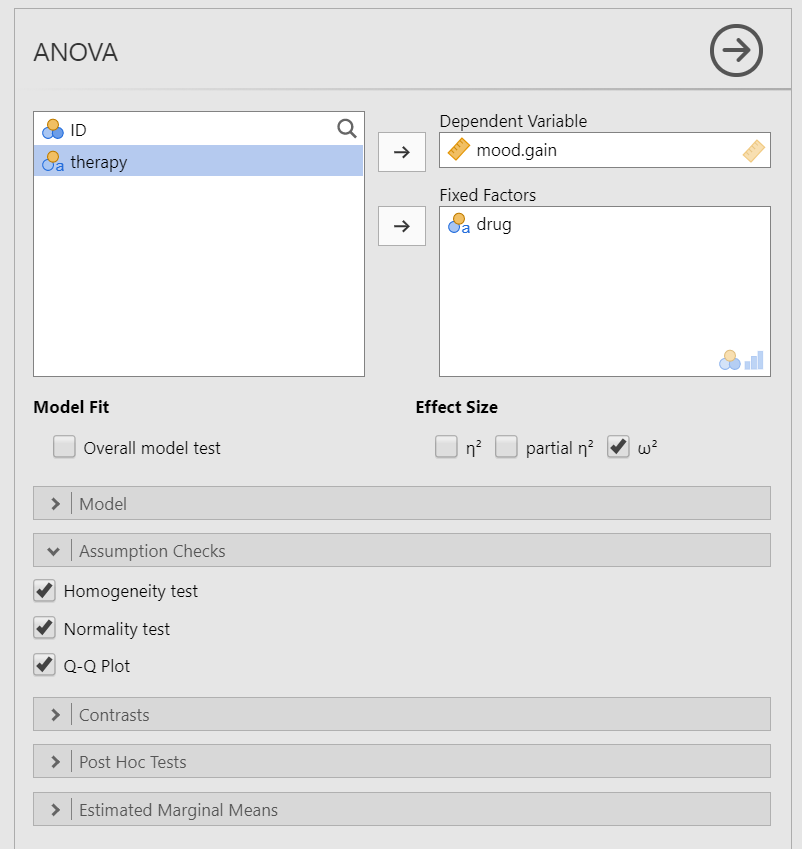
\includegraphics[width=0.8\linewidth]{images/04_one-way-anova/one-way_setup} 

}

\caption{One-way ANOVA setup in jamovi}\label{fig:unnamed-chunk-2}
\end{figure}

\hypertarget{checking-assumptions-in-jamovi-2}{%
\subsection{Checking assumptions in jamovi}\label{checking-assumptions-in-jamovi-2}}

We test for normality using the Shapiro-Wilk test and the Q-Q plot. The Shapiro-Wilk test was not statistically significant (W = .96, \emph{p} = .605); therefore, this indicates the data is normally distributed. Furthermore, the lines are fairly close to the diagonal line in the Q-Q plot. We can conclude that we satisfy the assumption of normality.

We test for homogeneity of variance using the Levene's test. The Levene's test was not statistically significant (\emph{F} {[}2, 15{]} = 1.45, \emph{p} = .266); therefore, this indicates our data satisfies the assumption of homogeneity of variance. However, I would add a caveat that we have a small sample of data (\emph{N} = 18); we should have tried to collect more data.

\begin{figure}

{\centering 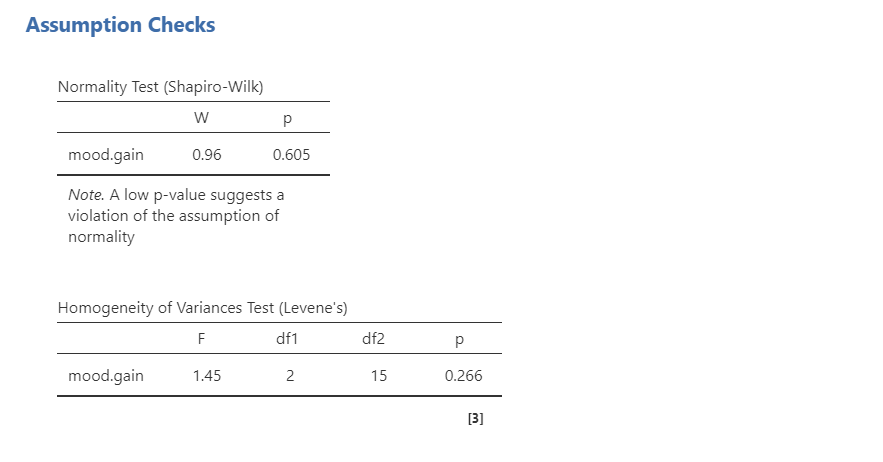
\includegraphics[width=1\linewidth]{images/04_one-way-anova/one-way_assumptions1} 

}

\caption{Testing assumptions in jamovi}\label{fig:unnamed-chunk-3}
\end{figure}

\begin{figure}

{\centering 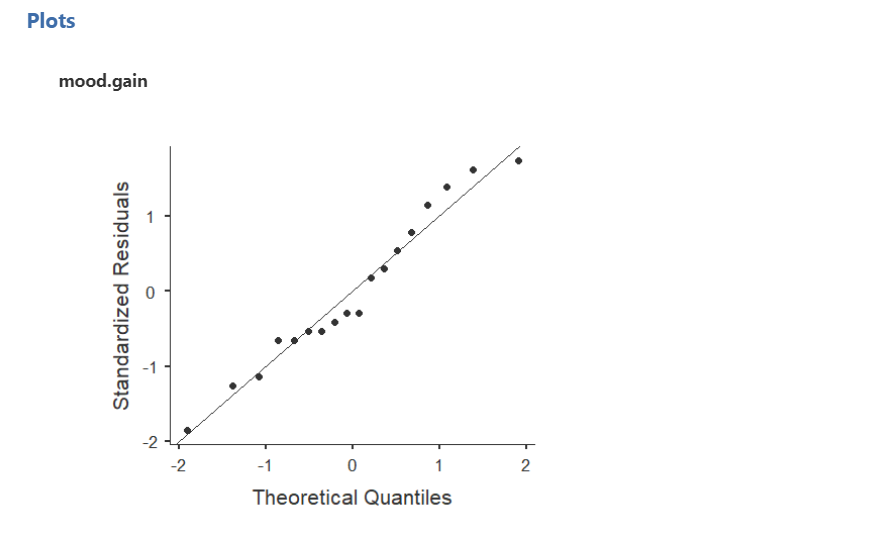
\includegraphics[width=1\linewidth]{images/04_one-way-anova/one-way_assumptions2} 

}

\caption{**CAPTION THIS FIGURE!!**}\label{fig:unnamed-chunk-4}
\end{figure}

\hypertarget{interpreting-results-2}{%
\section{Interpreting results}\label{interpreting-results-2}}

Once we are satisfied we have satisfied the assumptions for the one-way ANOVA, we can interpret our results.

\begin{figure}

{\centering 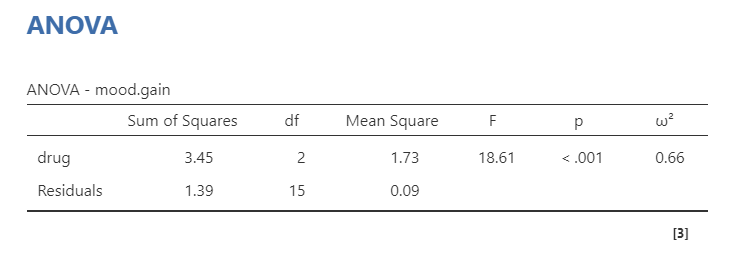
\includegraphics[width=1\linewidth]{images/04_one-way-anova/one-way_results} 

}

\caption{One-way ANOVA results in jamovi}\label{fig:unnamed-chunk-5}
\end{figure}

Our p-value is less than .05, so our results are statistically significant. We can write up our results in APA something like this:

\begin{quote}
There is a significant difference in mood gain across the three drug conditions, \emph{F} (2, 15) = 18.61, \emph{p} \textless{} .001, \(\omega^2\) = .66.
\end{quote}

Sometimes, people like to put the statistics inside a parentheses. In that case, you need to change the parentheses around the degrees of freedom as brackets. Here's another example write-up of the results in APA style:

\begin{quote}
There is a significant difference in mood gain across the three drug conditions (\emph{F} {[}2, 15{]} = 18.61, \emph{p} \textless{} .001, \(\omega^2\) = .66).
\end{quote}

\hypertarget{a-note-on-one-tailed-vs.-two-tailed-tests}{%
\subsection{A note on one-tailed vs.~two-tailed tests}\label{a-note-on-one-tailed-vs.-two-tailed-tests}}

Unlike a t-test, we would not halve the p-value in an F-ratio because it is an omnibus test. Our planned contrasts or post-hoc tests can tell us where differences are, and we can provide directional hypotheses there if we so choose.

\hypertarget{what-if-i-violated-assumptions-2}{%
\section{What if I violated assumptions?}\label{what-if-i-violated-assumptions-2}}

The great news is that jamovi includes the Welch's F-statistic and the Kruskal-Wallis non-parametric test! The bad news is that you lose some functionality in jamovi when you use them. Just like with the Welch's t-statistic (for the independent t-test), it does not have the assumption of equal variances so it's appropriate to use if your data is normally distributed but does not have homogeneous variances. Similarly, the Kruskal-Wallis test is the non-parametric version of the one-way ANOVA and should be used if you do not satisfy the assumption of normality.

Here's what statistic you should choose based on satisfying assumptions:

\begin{longtable}[]{@{}lll@{}}
\toprule
& \textbf{Normality: satisfied} & \textbf{Normality: not satisfied}\tabularnewline
\midrule
\endhead
\textbf{Homogeneity of Variance: satisfied} & one-way ANOVA & Kruskal-Wallis\tabularnewline
\textbf{Homogeneity of Variance: not satisfied} & Welch's F-test & Kruskal-Wallis\tabularnewline
\bottomrule
\end{longtable}

\hypertarget{welchs-f-test-in-jamovi}{%
\subsubsection{Welch's F-test in jamovi}\label{welchs-f-test-in-jamovi}}

To conduct this in jamovi, you will need to use the ``One-Way ANOVA'' test, not the ``ANOVA'' test. The unfortunate thing about this test is that it strangely does not provide effect sizes.

In jamovi, under Variances select \texttt{Don\textquotesingle{}t\ assume\ equal\ (Welch\textquotesingle{}s)}. Move \texttt{mood.gain} to the Dependent Variable box and \texttt{drug} to your Grouping Variable box. You will interpret the results similarly to the one-way ANOVA:

\begin{figure}

{\centering 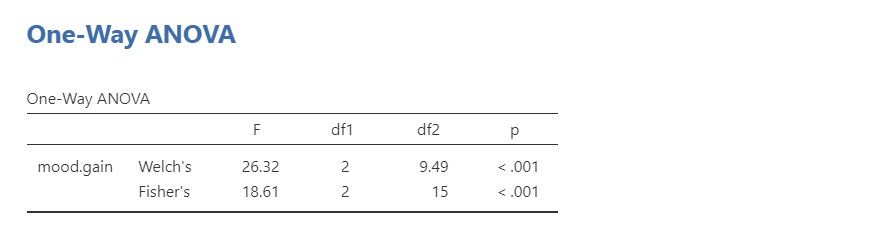
\includegraphics[width=1\linewidth]{images/04_one-way-anova/one-way_results_Welch} 

}

\caption{One-way ANOVA results in jamovi}\label{fig:unnamed-chunk-6}
\end{figure}

\begin{quote}
Using a Welch's F-test, there is a significant difference in mood gain across the three drug conditions, \emph{F} (2, 9.49) = 26.32, \emph{p} \textless{} .001.
\end{quote}

\hypertarget{kruskal-wallis-test-in-jamovi}{%
\subsubsection{Kruskal-Wallis test in jamovi}\label{kruskal-wallis-test-in-jamovi}}

To perform the Kruskal-Wallis test in jamovi, you will need to select under the ANOVA button ``One-Way ANOVA, Kruskal Wallis'' towards the bottom of the list of options. Move \texttt{mood.gain} to the Dependent Variables box and \texttt{drug} to the Grouping Variable box. Select Effect size; if you need post hoc comparisons select DSCF pairwise comparisons (see section below on group differences). You will interpret the results similarly to the one-way ANOVA:

\begin{figure}

{\centering 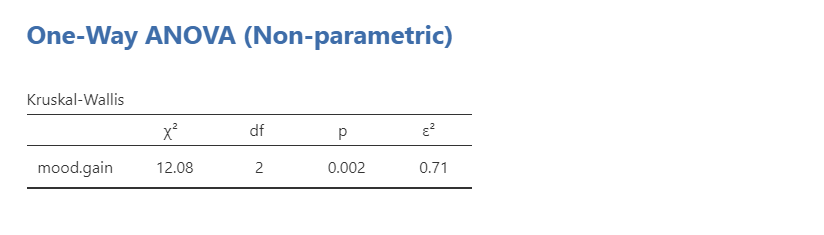
\includegraphics[width=1\linewidth]{images/04_one-way-anova/one-way_results_Kruskal} 

}

\caption{Kruskal-Wallis results in jamovi}\label{fig:unnamed-chunk-7}
\end{figure}

\begin{quote}
Using a Kruskal-Wallis test, there is a significant difference in mood gain across the three drug conditions, \(\chi^2\) (2) = 12.08, \emph{p} = .002, \(\epsilon^2\) = .71.
\end{quote}

Notice how in this case all three results converge and show there is a statistically significant difference in the results! The problem is\ldots{} differences in which groups?

\hypertarget{finding-group-differences}{%
\section{Finding Group Differences}\label{finding-group-differences}}

Often, we're not interested in just \emph{whether} there is a difference (which the F-statistic can tell us), but \emph{where} the differences are between groups (which the F-statistic cannot tell us). For that, we use either \underline{planned contrasts} when you have specific hypotheses you want to test or \underline{post-hoc comparisons} when you have no specific hypotheses.

\textbf{Note}: You \underline{do not} perform contrasts or post hoc comparisons if your overall \(F\) statistic is not statistically significant. You do not interpret group differences if you fail to reject the null hypothesis that there are no group differences!

\hypertarget{planned-contrasts}{%
\subsection{Planned Contrasts}\label{planned-contrasts}}

If you have before-analysis hypotheses of group differences in your data, you will use planned contrasts. You can find the planned contrasts in the ANOVA (but not the one-way ANOVA) setup as a drop-down menu. Note that while I show all six contrasts that jamovi provides, you do not normally do multiple contrasts. These are just shown for illustrative purposes:

\begin{enumerate}
\def\labelenumi{\arabic{enumi}.}
\tightlist
\item
  \textbf{Deviation}: compares the effect of each category (except the first category) to the overall experimental effect. The order of categories is alphabetical or numerical order. Notice how anxifree is considered the first category.
\end{enumerate}

\begin{figure}

{\centering 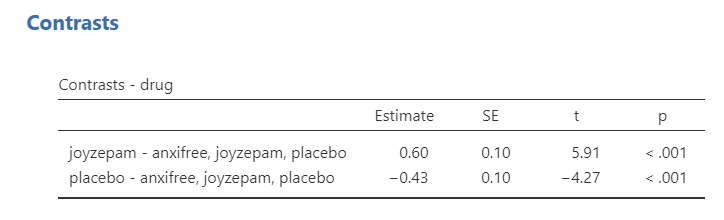
\includegraphics[width=1\linewidth]{images/04_one-way-anova/contrasts_deviation} 

}

\caption{**CAPTION THIS FIGURE!!**}\label{fig:unnamed-chunk-8}
\end{figure}

\begin{enumerate}
\def\labelenumi{\arabic{enumi}.}
\setcounter{enumi}{1}
\tightlist
\item
  \textbf{Simple}: Each category is compared to the first category. The order of categories is alphabetical or numerical order. Notice how anxifree is considered the first category.
\end{enumerate}

\begin{figure}

{\centering 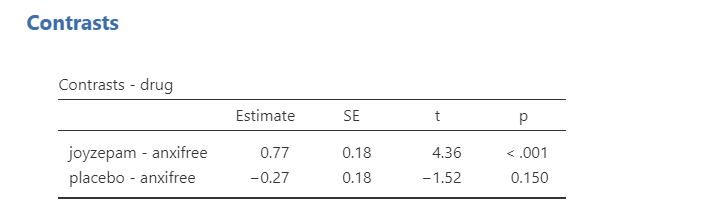
\includegraphics[width=1\linewidth]{images/04_one-way-anova/contrasts_simple} 

}

\caption{**CAPTION THIS FIGURE!!**}\label{fig:unnamed-chunk-9}
\end{figure}

\begin{enumerate}
\def\labelenumi{\arabic{enumi}.}
\setcounter{enumi}{2}
\tightlist
\item
  \textbf{Difference}: Each category (except the first) is compared to the mean effect of all previous categories.
\end{enumerate}

\begin{figure}

{\centering 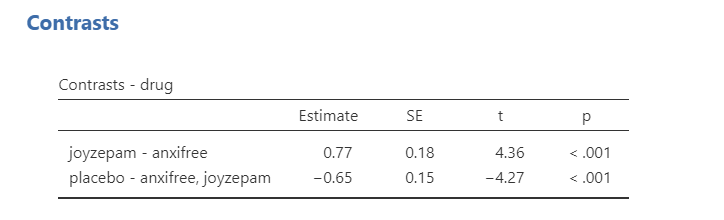
\includegraphics[width=1\linewidth]{images/04_one-way-anova/contrasts_difference} 

}

\caption{**CAPTION THIS FIGURE!!**}\label{fig:unnamed-chunk-10}
\end{figure}

\begin{enumerate}
\def\labelenumi{\arabic{enumi}.}
\setcounter{enumi}{3}
\tightlist
\item
  \textbf{Helmert}: Each category (except the last) is compared to the mean effect of all subsequent categories.
\end{enumerate}

\begin{figure}

{\centering 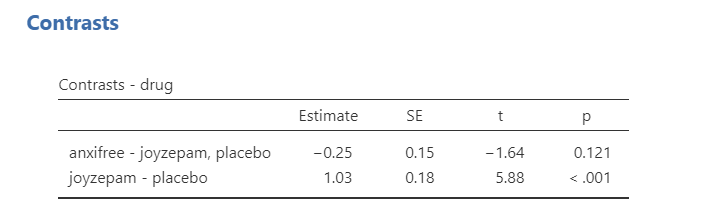
\includegraphics[width=1\linewidth]{images/04_one-way-anova/contrasts_helmert} 

}

\caption{**CAPTION THIS FIGURE!!**}\label{fig:unnamed-chunk-11}
\end{figure}

\begin{enumerate}
\def\labelenumi{\arabic{enumi}.}
\setcounter{enumi}{4}
\tightlist
\item
  \textbf{Repeated}: Each category is compared to the last category.
\end{enumerate}

\begin{figure}

{\centering 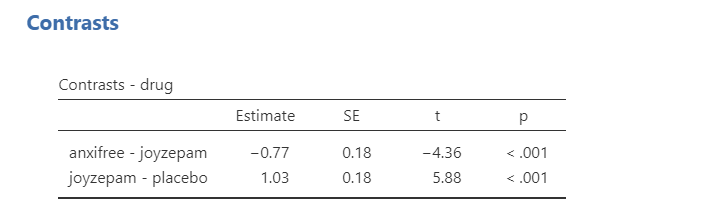
\includegraphics[width=1\linewidth]{images/04_one-way-anova/contrasts_repeated} 

}

\caption{**CAPTION THIS FIGURE!!**}\label{fig:unnamed-chunk-12}
\end{figure}

\begin{enumerate}
\def\labelenumi{\arabic{enumi}.}
\setcounter{enumi}{5}
\tightlist
\item
  \textbf{Polynomial}: Tests trends in the data. It will examine the \emph{n-1}\textsuperscript{th} degree based on the number of groups. In this case, because we have 3 groups it is testing both a linear (\textsuperscript{1}) and quadratic (\textsuperscript{2}) trend. If we had 5 groups, it would test a linear (\textsuperscript{1}), quadratic (\textsuperscript{2}), cubic (\textsuperscript{3}), and quartic (\textsuperscript{4}) trend. Note that your factor levels must be ordinal for a polynomial contrast to make sense.
\end{enumerate}

\begin{figure}

{\centering 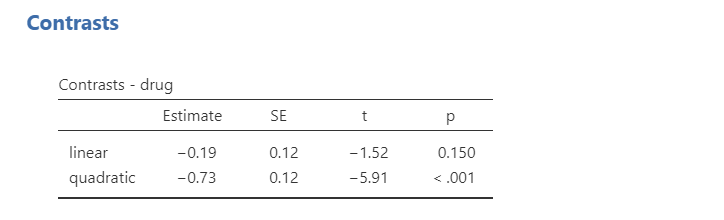
\includegraphics[width=1\linewidth]{images/04_one-way-anova/contrasts_polynomial} 

}

\caption{**CAPTION THIS FIGURE!!**}\label{fig:unnamed-chunk-13}
\end{figure}

\textbf{Test yourself!} Which contrast would make \underline{most sense} to test given that we want to know how our drug compares to the other two drugs? deviation simple difference helmert repeated polynomial

\hypertarget{writing-up-planned-contrasts}{%
\subsubsection{Writing up planned contrasts}\label{writing-up-planned-contrasts}}

Here's some example write-ups of the above results.

\begin{quote}
There is a significant difference in mood gain across the three drug conditions, \emph{F} (2, 15) = 18.61, \emph{p} \textless{} .001. Repeated contrasts showed that \emph{Joyzepam} (\emph{M} = 1.48, \emph{SD} = .21) outperformed both \emph{Anxifree} (\emph{M} = .72, \emph{SD} = .39; \emph{p} \textless{} .001) and the placebo condition (\emph{M} = .45, \emph{SD} = .28; \emph{p} \textless{} .001).

(Note how this example makes no sense because our data is not ordinal) There is a significant difference in mood gain across the three drug conditions, \emph{F} (2, 15) = 18.61, \emph{p} \textless{} .001. There was not a significant linear trend across the drug conditions (\emph{p} = .150).
\end{quote}

\hypertarget{post-hoc-comparisons}{%
\subsection{Post hoc comparisons}\label{post-hoc-comparisons}}

Often, we do not have any \emph{a priori} (or planned) predictions or hypotheses about our group differences. In this case, we use post hoc procedures. These procedures do \underline{pairwise comparisons} among all of our groups, like t-tests across each of our groups. As we noted on the first page of this handout, this can be highly problematic for our Type I error rate! Therefore, we must perform corrections to control our familywise error rate.

jamovi currently supports five types of post-hoc tests; I generally only use Tukey or Bonferonni:

\begin{enumerate}
\def\labelenumi{\arabic{enumi}.}
\tightlist
\item
  \textbf{No correction}: This doesn't correct for a Type I error at all. Don't use this! I won't even show it. It's bad. Never use it. NEVER. You are warned!
\item
  \textbf{Tukey}: This is the post hoc test I use most often. It controls the Type I error rate well, but isn't as conservative of a control as the Bonferonni.
\item
  \textbf{Scheffe}: Honestly, I've never used it. I am not sure how it's calculated.
\item
  \textbf{Bonferroni}: This is the most conservative test. It's good if you only have a small number of comparisons to make or if you \emph{really} want to control your Type I error rate. If you have a lot of them to test , then you should use something else.
\item
  \textbf{Holm}: Honestly, I've never used it. I am not sure how it's calculated.
\end{enumerate}

Games-Howell for when you have unequal variances and Tukey for when you have equal variances. They will each calculate your p-values slightly differently but in a way to control for our Type I error rate as best it can. They are interpreted very similarly, so we will proceed with the Tukey's post hoc comparisons because we satisfied the assumption of equal variances.

To request post hoc tests from the one-way ANOVA, open the collapsed menu at the bottom of the setup menu. Select \texttt{Tukey\ (equal\ variances} under Post-Hoc Test and select \texttt{Mean\ difference}, \texttt{Report\ significance}, and \texttt{Flag\ significant\ comparisons} under Statistics. Optionally, you can request the \texttt{Test\ results\ (t\ and\ df)} although this is not necessary.

Below shows the post hoc test results for our one-way ANOVA. Notice the differences in p-values across the four post hoc tests and how all other values are the same. Notice how the Bonferroni is most conservative (i.e., has the largest p-values) and the Holm's is the least conservative (i.e., has the smallest p-values). Keep in mind you do not normally ask for multiple post hoc comparisons. Just pick one! Normally, I just pick Tukey's.

\begin{figure}

{\centering 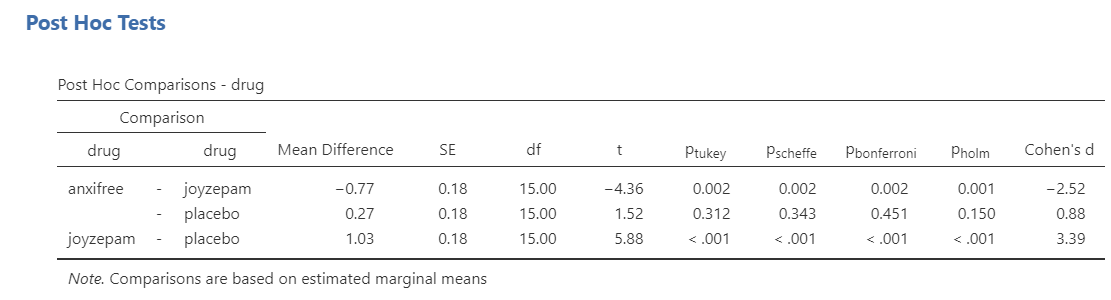
\includegraphics[width=1\linewidth]{images/04_one-way-anova/one-way_results_post-hoc} 

}

\caption{Post hoc test results in jamovi}\label{fig:unnamed-chunk-14}
\end{figure}

\hypertarget{writing-up-post-hoc-results}{%
\subsubsection{Writing up post hoc results}\label{writing-up-post-hoc-results}}

The way we would write up each of the post hoc comparisons is very similar. Given that I usually use Tukey, here is a write-up for those results:

\begin{quote}
There is a significant difference in mood gain across the three drug conditions, \emph{F} (2, 15) = 18.61, \emph{p} \textless{} .001. Post hoc comparisons using Tukey's HSD revealed that our drug \emph{Joyzepam} (\emph{M} = 1.48, \emph{SD} = .21) outperformed both \emph{Anxifree} (\emph{M} = .72, \emph{SD} = .39; \emph{p} = .002) and the placebo condition (\emph{M} = .45, \emph{SD} = .28; \emph{p} \textless{} .001); there were no differences between \emph{Anxifree} and the placebo condition (\emph{p}
\end{quote}

\hypertarget{group-differences-with-violated-assumptions}{%
\subsection{Group differences with violated assumptions}\label{group-differences-with-violated-assumptions}}

If you are using Welch's F-test using the One-Way ANOVA in jamovi, you should select under Post-Hoc Tests \texttt{Games-Howell\ (unequal\ variances)}. These will be interpreted similarly to the post hoc comparisons above.

If you are using the Kruskal-Wallis test, you will select the check-box for \texttt{DSCF\ pairwise\ comparisons}. This stands for the Dwass-Steel-Critchlow-Fligner test. All you need to know is that they, too, are interpreted similarly to the post hoc comparisons above.

Unfortunately, you cannot perform contrasts with either the Welch's F-test or Kruskal-Wallis test.

\hypertarget{relationship-between-anova-and-t-test}{%
\section{Relationship between ANOVA and t-test}\label{relationship-between-anova-and-t-test}}

An ANOVA with two groups is identical to the t-test. That means the F and t statistics are directly related, and you will get the same p-value. For example, imagine you run a t-test and get a t-statistic of \emph{t} (16) = -1.31, \emph{p} = .210. If you ran it as a one-way ANOVA, you would get an F-statistic of \emph{F} (1, 16) = 1.71, \emph{p} = .210.

\(F = t^2\)

\(t = \sqrt{F}\)

Just a fun little bit of trivia! So if you accidentally do an F-test with two groups, no need to go back and redo the analyses (although you should if you are sharing your code for reproducibility). You can just convert your F to a t statistic easily!

\hypertarget{tips-on-writing-up-results}{%
\section{Tips on writing up results}\label{tips-on-writing-up-results}}

Writing up results in APA style is both a science and an art. There's a science to what you need to report. For example, you always report the statistics exactly the same: \emph{F} (df\textsubscript{WG}, df\textsubscript{BG}) = X.XX, \emph{p} = .XXX. You also always report the group means (\emph{M}) and standard deviations (\emph{SD}), although you can report them in-text like I did above or in a descriptives table like you can ask from jamovi.

However, there's also an art to it. Notice how I wrote that up in a way to summarize the findings as succinctly as possible. I could have said there was a difference between \emph{anxifree} and \emph{joyzepam} and a difference between \emph{joyzepam} and the placebo, but that's a lot more words and isn't written in a way to focus on what I'm hoping to see: that my drug \emph{joyzepam} performed better than the competitor \emph{anxifree} and a placebo condition.

This is where you need to think creatively and be very critical in checking that what you say makes sense. Read your write-ups carefully! Have someone else read it. Can they understand what you mean?

\hypertarget{your-turn-2}{%
\section{Your turn!}\label{your-turn-2}}

Open the \texttt{Sample\_Dataset\_2014.xlsx} file that we will be using for all Your Turn exercises.

Perform one-way ANOVAs based on the following research questions. Check your assumptions and ensure you are using the correct tests.

To get the most out of these exercises, try to first find out the answer on your own and then use the drop-down menus to check your answer.

\begin{enumerate}
\def\labelenumi{\arabic{enumi}.}
\item
  \textbf{Does students differ on English scores by rank (i.e., freshmen, sophomore, junior, senior)?}

  \begin{itemize}
  \item
    Do you satisfy the assumption of normality? yes no
  \item
    Do you satisfy the assumption of homogeneity of variance? yes no
  \item
    Which statistic should you use? one-way ANOVA Welch's F-test Kruskal-Wallis test
  \item
    Do students differ on English scores by rank? yes no
  \item
    Should you perform a planned contrast or post hoc comparison? yes no
  \item
    What are the results of the post hoc comparison? N/A - Don't perform Freshmen had higher English scores than sophomores, juniors, and seniors Freshmen and sophomores had higher English scores than juniors and seniors
  \end{itemize}
\item
  \textbf{Does smoking status (Smoking: Nonsmoker = 0, Past smoker = 1, Current smoker = 2) relate to sprint time?}

  \begin{itemize}
  \item
    Do you satisfy the assumption of normality? yes no
  \item
    Do you satisfy the assumption of homogeneity of variance? yes no
  \item
    Which statistic should you use? one-way ANOVA Welch's F-test Kruskal-Wallis test
  \item
    Does smoking status relate to sprint time? yes no
  \item
    Should you perform a planned contrast or post hoc comparison? yes no
  \item
    What are the results of the post hoc comparison? N/A - Don't perform Nonsmokers had significantly faster sprint times than current smokers Nonsmokers and past smokers had significantly faster spring times than current smokers Nonsmokers had significantly faster sprint times than both past and current smokers
  \end{itemize}
\end{enumerate}

\hypertarget{repeated-measures-anova}{%
\chapter{Repeated Measures ANOVA}\label{repeated-measures-anova}}

\hypertarget{what-is-the-repeated-measures-anova}{%
\section{What is the repeated measures ANOVA?}\label{what-is-the-repeated-measures-anova}}

The repeated measures analysis of variance (ANOVA) is used to test the difference in our dependent variable between \underline{three or more} groups of observations in which all participants participate in all groups or levels. Our grouping variable is our independent variable. In other words, we use the one-way ANOVA when we have a research question with a \textbf{continuous dependent variable} and a \textbf{categorical independent variable with three or more categories in which the same participants are in each category}.

The repeated measures ANOVA is also sometimes called the one-way related ANOVA.

There are two ways we could have the repeated measures ANOVA. Perhaps the same group of participants are measured in the same dependent variable at three or more time points. In this case, our independent variable is time and our dependent variable is whatever is measured at each time point.

\begin{figure}

{\centering 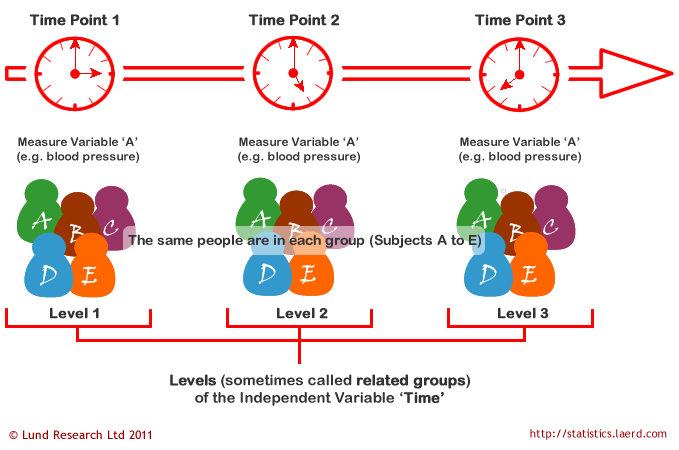
\includegraphics[width=0.8\linewidth]{images/05-repeated-measures-anova/Laerd1} 

}

\caption{Repeated measures ANOVA by Time}\label{fig:unnamed-chunk-1}
\end{figure}

The other way we might have the repeated measures ANOVA is if all our participants participate in all conditions of our study. In this case, our independent variable is the treatment or condition and the dependent variable is whatever is measured in each treatment or condition.

\begin{figure}

{\centering 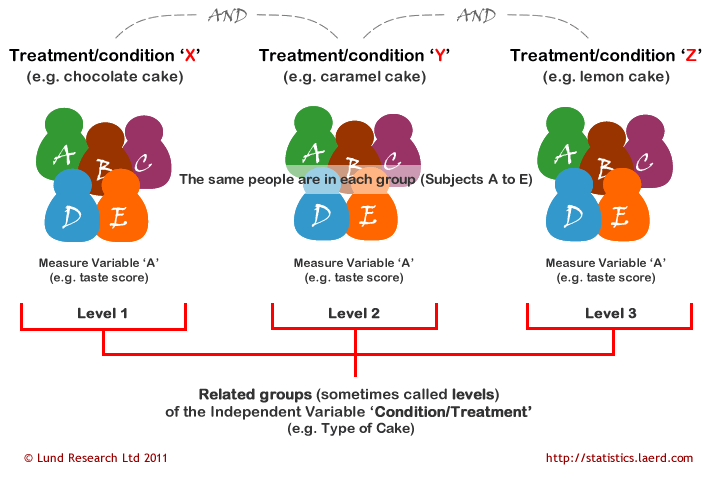
\includegraphics[width=0.8\linewidth]{images/05-repeated-measures-anova/Laerd2} 

}

\caption{Repeated measures ANOVA by Conditions}\label{fig:unnamed-chunk-2}
\end{figure}

\hypertarget{data-set-up-3}{%
\section{Data set-up}\label{data-set-up-3}}

To conduct the repeated measures ANOVA, we first need to ensure our data is set-up properly in our dataset. This requires having two columns: one with our continuous dependent variable and one indicating which group the participant is in. Each row is a unique participant or unit of analysis. Here's what example data may look like if we were testing for differences in a test score by students in my fall, spring, or summer semesters of my course in which three participants are in each of my three courses.

\begin{longtable}[]{@{}llll@{}}
\caption{Example data for the repeated measures ANOVA}\tabularnewline
\toprule
ID & Fall & Spring & Summer\tabularnewline
\midrule
\endfirsthead
\toprule
ID & Fall & Spring & Summer\tabularnewline
\midrule
\endhead
1 & 86 & 79 & 90\tabularnewline
2 & 80 & 82 & 72\tabularnewline
3 & 75 & 84 & 75\tabularnewline
\bottomrule
\end{longtable}

In the example data above, what is your \textbf{independent variable}? ID Semester TestScore

In the example data above, what is your \textbf{dependent variable}? ID Semester TestScore

\hypertarget{the-math-behind-the-repeated-measures-anova}{%
\section{The math behind the repeated measures ANOVA}\label{the-math-behind-the-repeated-measures-anova}}

The basic math of the repeated measures ANOVA is very similar to the one-way ANOVA except that the \(SS_{WG}\) is partitioned into two parts. Since there are the same subjects in each group, we can remove the variability due to the individual differences between subjects from the within-groups variability.

\(F = \frac{BG \:variance}{WG \:variance} = \frac{MS_{BG}}{MS_{WG}} = \frac{\frac{SS_{BG}}{df_{BG}}}{\frac{SS_{WG}}{df_{WG}}}\)

So whereas our denominator in the one-way ANOVA has \(SS_{WG}\), our denominator for the repeated measures ANOVA has \(SS_{WG}-SS_{subjects}\). You can see this in more detail in the figure below by Laerd Statistics. The one-way ANOVA (also known as the independent samples ANOVA) splits the total variability in scores by the between-group (conditions) variability and the within-groups (error) variability. The repeated measures anova takes that within-groups variability and splits out the subject variability from the error variability.

\begin{figure}

{\centering 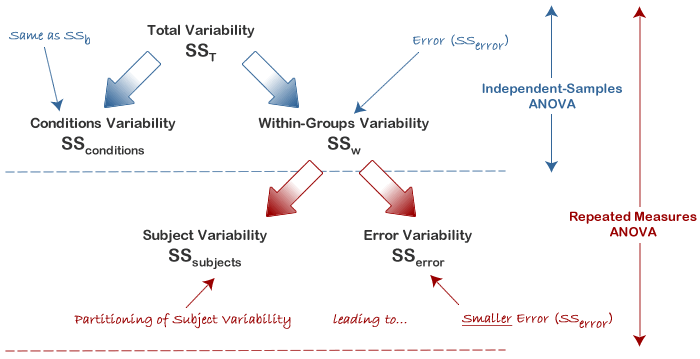
\includegraphics[width=0.8\linewidth]{images/05-repeated-measures-anova/Laerd3} 

}

\caption{Repeated measures ANOVA by Time}\label{fig:unnamed-chunk-3}
\end{figure}

I won't go into any more detail on the math of the repeated measures ANOVA, but you can read more on Laerd Statistics \href{https://statistics.laerd.com/statistical-guides/repeated-measures-anova-statistical-guide-2.php}{guide for the repeated measures ANOVA}.

\hypertarget{assumptions-2}{%
\section{Assumptions}\label{assumptions-2}}

As a parametric test, the repeated measures ANOVA has the same assumptions as other parametric tests:

\begin{enumerate}
\def\labelenumi{\arabic{enumi}.}
\item
  The dependent variable is \textbf{normally distributed}
\item
  Variances in the two groups are roughly equal (i.e., \textbf{homogeneity of variances}); in repeated measures ANOVA this is called the assumption of \textbf{sphericity}
\item
  The dependent variable is \textbf{interval or ratio} (i.e., continuous)
\item
  \sout{Scores are \textbf{independent} between groups} (this assumption is not relevant because all participants participate in all conditions)
\end{enumerate}

We cannot \underline{test} the third and fourth assumptions; rather, those are based on knowing your data. However, we can and should test for the first two assumptions. Fortunately, the one-way ANOVA in jamovi has three check boxes under ``Assumption Checks'' that lets us test for both assumptions.

\hypertarget{sphericity-assumption}{%
\subsection{Sphericity Assumption}\label{sphericity-assumption}}

The sphericity assumption is essentially the repeated measures ANOVA equivalent of homogeneity of variances. Sphericity means there is equality of variances of the \emph{differences} between treatment levels. For example, if there are three groups, then the difference in all three pairs of differences (1-2, 1-3, 2-3) need to have approximately equal variances. You only need to care about sphericity when there are at least three conditions, which is why we did not talk about this with the dependent t-test.

Fortunately, like the other assumption checks, testing for sphericity is as simple as a checkbox in jamovi.

\hypertarget{in-jamovi-2}{%
\section{In jamovi}\label{in-jamovi-2}}

Let's run an example with data from lsj-data. Open data from your Data Library in ``lsj-data''. Select and open ``broca''.

This dataset is hypothetical data in which six patients suffering from Broca's Aphasia (a language deficit commonly experienced following a stroke) complete three word recognition tasks. On the first (speech production) task, patients were required to repeat single words read out aloud by the researcher. On the second (conceptual) task, designed to test word comprehension, patients were required to match a series of pictures with their correct name. On the third (syntax) task, designed to test knowledge of correct word order, patients were asked to reorder syntactically incorrect sentences. Each patient completed all three tasks. The order in which patients attempted the tasks was counterbalanced between participants. Each task consisted of a series of 10 attempts. The number of attempts successfully completed by each patient are provided in the dataset.

\begin{enumerate}
\def\labelenumi{\arabic{enumi}.}
\item
  To perform a repeated measures ANOVA in jamovi, go to the Analyses tab, click the ANOVA button, and choose ``Repeated Measures ANOVA''.
\item
  Under ``Repeated Measures Factors'' name your independent variable. In this case you can name it ``Task''. Rename the three levels of Task: Speech, Conceptual, and Syntax.
\item
  Under ``Repeated Measures Cells'' move the given variable into the correct level. For example, you'll move Speech to the Speech cell.
\item
  Select Generalised \(\eta^2\) as your measure of effect size.
\item
  In the Assumption Checks drop-down menu, select \texttt{Sphericity\ tests}. You'll note that if you violate the assumption of sphericity, there are two corrections provided. These will be discussed later.
\item
  In the Post Hoc Tests drop-down menu, select \texttt{Tukey}. Remember that we only interpret these if the overall \emph{F} is statistically significant.
\item
  In the Estimated Marginal Means drop-down menu, move Task to the Marginal Means box, select \texttt{Marginal\ means\ tables}, and select \texttt{Observed\ scores} . Uncheck \texttt{Equal\ cell\ weights}.
\end{enumerate}

When you are done, your setup should look like this:

\begin{figure}

{\centering 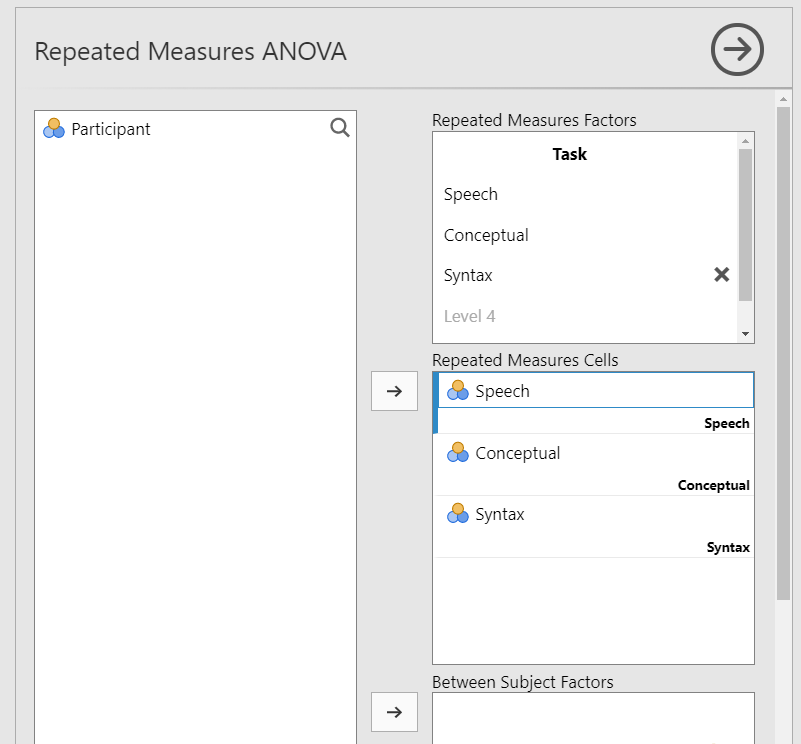
\includegraphics[width=0.8\linewidth]{images/05-repeated-measures-anova/rm-anova_setup1} 

}

\caption{Repeated Measures ANOVA setup in jamovi}\label{fig:unnamed-chunk-4}
\end{figure}

\begin{figure}

{\centering 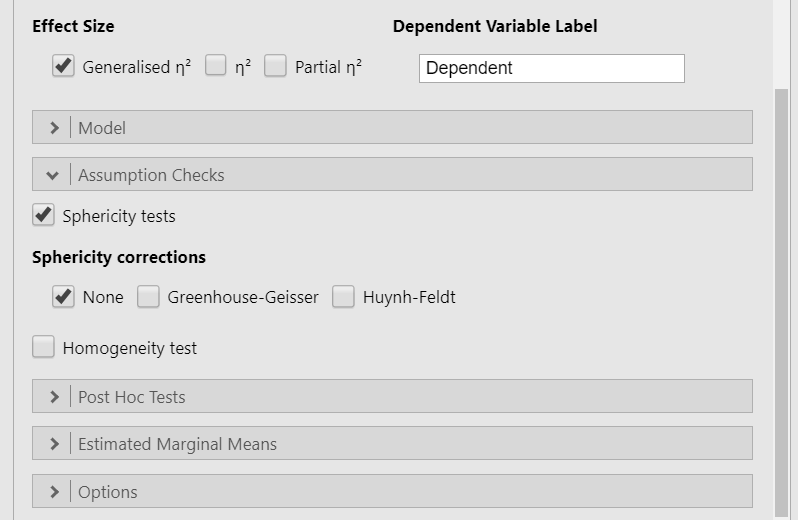
\includegraphics[width=0.8\linewidth]{images/05-repeated-measures-anova/rm-anova_setup2} 

}

\caption{Repeated Measures ANOVA setup in jamovi}\label{fig:unnamed-chunk-5}
\end{figure}

\hypertarget{checking-assumptions-in-jamovi-3}{%
\subsection{Checking assumptions in jamovi}\label{checking-assumptions-in-jamovi-3}}

You'll notice there are no options to check for normality in the repeated measures ANOVA in jamovi. There's an \href{https://forum.jamovi.org/viewtopic.php?f=5\&t=1045}{interesting conversation} on the topic in the jamovi forums. Suffice to say, it's complicated and maybe someday they will implement it. For now, we just won't worry about it for the repeated measures ANOVA.

So what we need to worry about is testing our assumption of sphericity. You should have checked the box \texttt{Sphericity\ tests} under the Assumption Checks drop-down menu. That produces the following output:

\begin{figure}

{\centering 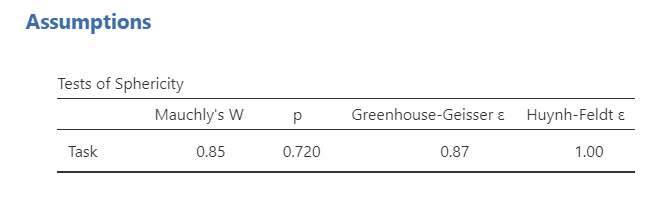
\includegraphics[width=1\linewidth]{images/05-repeated-measures-anova/rm-anova_sphericity} 

}

\caption{Testing sphericity in jamovi}\label{fig:unnamed-chunk-6}
\end{figure}

Mauchly's test of sphericity tests the null hypothesis that the variances of the differences between the conditions are equal. Therefore, just like with our previous assumption checks, if Mauchly's test is non-significant (i.e., \emph{p} \textgreater{} .05, as is the case in this analysis) then it is reasonable to conclude that the variances of the differences are not significantly different. This means we satisfy the assumption of sphericity and can conclude that the variances of the differences are roughly equal.

If Mauchly's test had been statistically significant (\emph{p} \textless{} .05), then we would conclude that the assumption had \emph{not} been met. In this case, we should apply a correction to the \emph{F}-value obtained in the repeated measures ANOVA:

\begin{itemize}
\tightlist
\item
  If the Greenhouse-Geisser value in the ``Tests of Sphericity'' table is \textgreater{} .75 then you should use the Huynh-Feldt correction.
\item
  If the Greenhouse-Geisser value is \textless{} .75, then you should use the Greenhouse-Geisser correction.
\end{itemize}

You can select these corrections in the Assumption Checks drop-down menu.

\hypertarget{interpreting-results-3}{%
\section{Interpreting results}\label{interpreting-results-3}}

Once we are satisfied we have satisfied the assumptions for the repeated measures, we can interpret our results.

\begin{figure}

{\centering 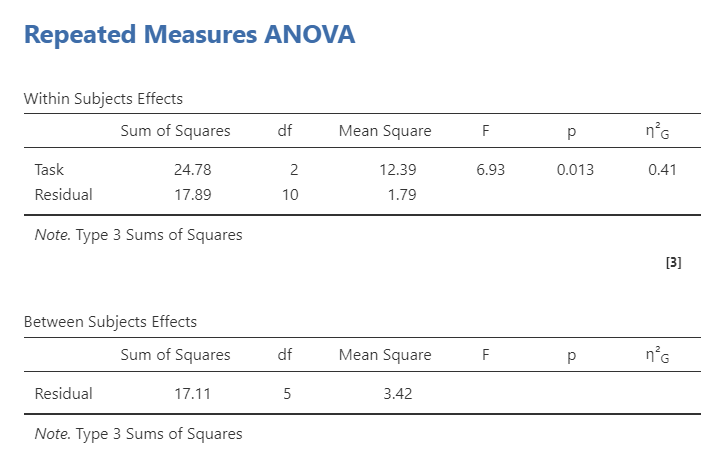
\includegraphics[width=1\linewidth]{images/05-repeated-measures-anova/rm-anova_results} 

}

\caption{One-way ANOVA results in jamovi}\label{fig:unnamed-chunk-7}
\end{figure}

You'll notice that jamovi provides you both a Within Subjects Effects table and Between Subjects Effects table. However, we only have a within-subjects effect (Task). Why did it give us a between-subjects table? With the repeated-measures ANOVA (which only has within-subjects IVs), this is just our \(SS_{BG}\). However, because we don't have one, it's not calculating anything. We can ignore it. It is only useful if we are conducting a mixed factorial ANOVA with both between-subjects and within-subjects effects.

Therefore, the Within Subjects Effects table is of most use to us. We can see that the overall effect of Task is statistically significant (\emph{p} = .013). Therefore we can look at our Post Hoc Tests results.

\begin{figure}

{\centering 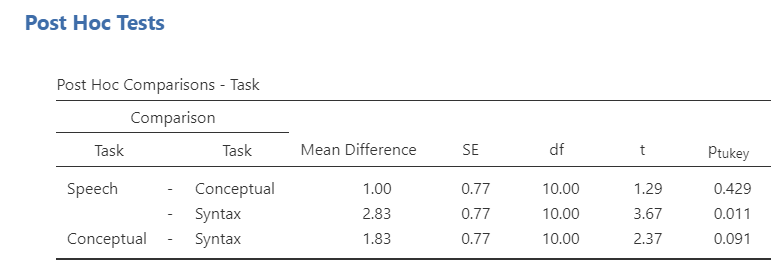
\includegraphics[width=1\linewidth]{images/05-repeated-measures-anova/rm-anova_tukey} 

}

\caption{One-way ANOVA results in jamovi}\label{fig:unnamed-chunk-8}
\end{figure}

The Tukey post hoc differences show that there was a significant difference between speech and syntax (\emph{p} = .011), but not between conceptual and both speech and syntax. Last, we can look at the Estimated Marginal Means - Task table to see the group means for reporting purposes. This shows us that participants recognized significantly more words in the speech task than in the syntax task.

We can write this up in APA style similar to the one-way ANOVA.

\begin{quote}
A repeated measures ANOVA was performed examining how three tasks affected word recognition in patients suffering from Broca's Aphasia. Task significantly affected word recall, \emph{F} (2, 10) = 6.93, \emph{p} = .013, \(\eta^2_G\) = .41. Tukey's post hoc difference tests indicated that participants recognized significantly more words in the speech task (\emph{M} = 7.17, \emph{SE} = .62) than participants in the syntax task (\emph{M} = 4.33, \emph{SE} = .62; \emph{p}~= .011). There were no differences between the conceptual task (\emph{M} = 6.17, \emph{SE} = .62) and both the speech and syntax tasks.
\end{quote}

\hypertarget{what-if-i-violated-assumptions-3}{%
\section{What if I violated assumptions?}\label{what-if-i-violated-assumptions-3}}

We have already discussed what to do if you violate the assumption of sphericity above; you select one of the two sphericity corrections.

If you violate the assumption of normality or if the dependent variable is ordinal, then you can use the Friedman test. You can select this using the Repeated Measures ANOVA - Friedman option under the ANOVA analysis.

Friedman's test can only examine one within-subjects variable, so you will move all three conditions (Speech, Conceptual, and Syntax) to the Measures box. Select \texttt{Pairwise\ comparisons\ (Durbin-Conover} for post hoc comparisons and \texttt{Descriptives} for the Means and Medians. Optionally, you can select to plot either the Means or Medians. The Setup is shown below.

\begin{figure}

{\centering 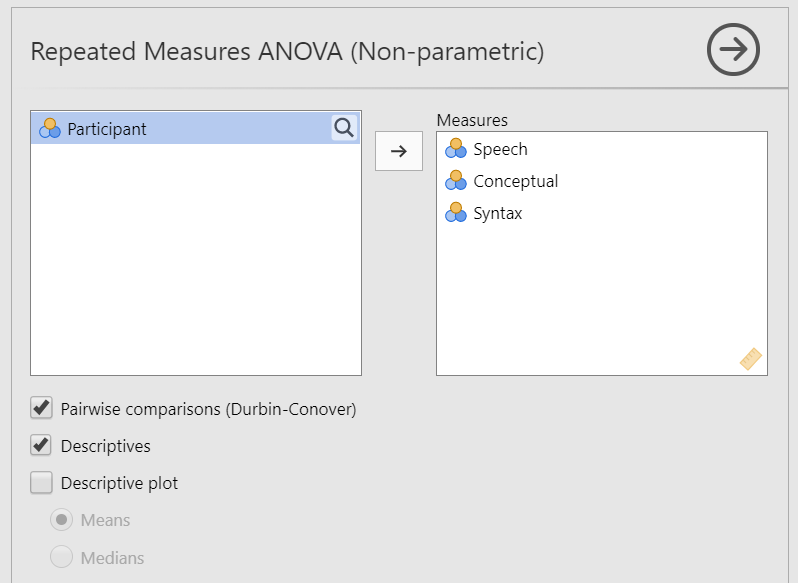
\includegraphics[width=0.8\linewidth]{images/05-repeated-measures-anova/rm-anova_friedman_setup} 

}

\caption{Repeated Measures ANOVA setup in jamovi}\label{fig:unnamed-chunk-9}
\end{figure}

Once you've set-up the analysis, you can interpret the results. Overall, we continue to see a statistically significant result and that there is only a significant difference between speech and syntax.

\begin{figure}

{\centering 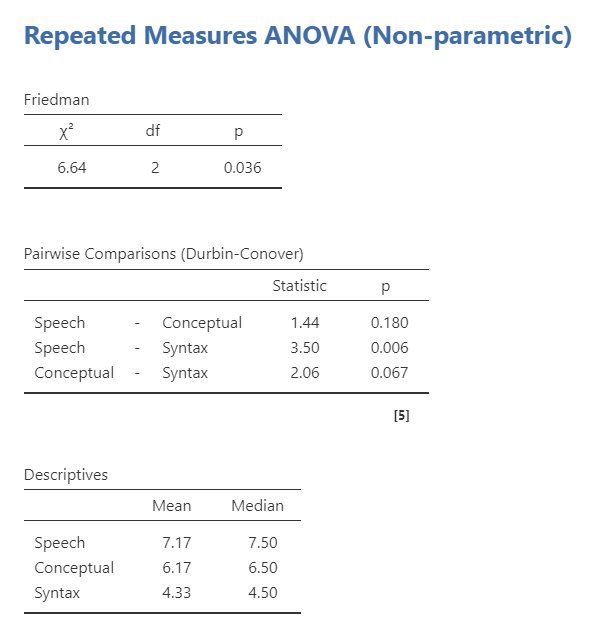
\includegraphics[width=1\linewidth]{images/05-repeated-measures-anova/rm-anova_friedman} 

}

\caption{Repeated Measures ANOVA setup in jamovi}\label{fig:unnamed-chunk-10}
\end{figure}

We can write up the results similarly as before:

\begin{quote}
Friedman's test was performed examining how three tasks affected word recognition in patients suffering from Broca's Aphasia. Task significantly affected word recall, \(\chi^2\) (2) = 6.64, \emph{p} = .036. Pairwise comparisons using Durbin-Conover indicated that participants recognized significantly more words in the speech task (\emph{M} = 7.17, \emph{Mdn} = 7.50) than participants in the syntax task (\emph{M} = 4.33, \emph{Mdn} = 6.50; \emph{p}~= .006). There were no differences between the conceptual task (\emph{M} = 6.17, \emph{Mdn} = 6.50) and both the speech and syntax tasks.
\end{quote}

\hypertarget{tips-on-writing-up-results-1}{%
\section{Tips on writing up results}\label{tips-on-writing-up-results-1}}

Writing up results in APA style is both a science and an art. There's a science to what you need to report. For example, you always report the statistics exactly the same: \emph{F} (df\textsubscript{WG}, df\textsubscript{BG}) = X.XX, \emph{p} = .XXX. You also always report the group means (\emph{M}) and standard deviations (\emph{SD}), although you can report them in-text like I did above or in a descriptives table like you can ask from jamovi.

However, there's also an art to it. Notice how I wrote that up in a way to summarize the findings as succinctly as possible. I could have said there was a difference between \emph{anxifree} and \emph{joyzepam} and a difference between \emph{joyzepam} and the placebo, but that's a lot more words and isn't written in a way to focus on what I'm hoping to see: that my drug \emph{joyzepam} performed better than the competitor \emph{anxifree} and a placebo condition.

This is where you need to think creatively and be very critical in checking that what you say makes sense. Read your write-ups carefully! Have someone else read it. Can they understand what you mean?

\hypertarget{your-turn-3}{%
\section{Your turn!}\label{your-turn-3}}

Open the \texttt{Sample\_Dataset\_2014.xlsx} file that we will be using for all Your Turn exercises.

Perform a repeated measures ANOVA based on the following research questions. Check your assumptions and ensure you are using the correct tests.

To get the most out of these exercises, try to first find out the answer on your own and then use the drop-down menus to check your answer.

\begin{enumerate}
\def\labelenumi{\arabic{enumi}.}
\item
  \textbf{Does students differ on their test scores (English, Reading, Math, Writing)?}

  \begin{itemize}
  \item
    Based on your understanding of the nature of the test scores, which statistic should you use? repeated measures ANOVA Friedman's test
  \item
    Should you apply a sphericity correction? If so, which one? N/A - using Friedman's test no, assumption satisfed yes, Greenhouse-Geisser yes, Huynh-Feldt
  \item
    Do students differ on their test scores? yes no
  \item
    Should you perform a planned contrast or post hoc comparison? yes no
  \item
    What are the results of the post hoc comparison? N/A - Don't perform All test scores were significantly different from one another All test scores were significantly different from one another except for English and Reading
  \end{itemize}
\end{enumerate}

\hypertarget{factorial-anova}{%
\chapter{Factorial ANOVA}\label{factorial-anova}}

\hypertarget{what-is-factorial-anova}{%
\section{What is factorial ANOVA?}\label{what-is-factorial-anova}}

Factorial ANOVA allows us to examine two or more independent variables (IVs) simultaneously. There are several types of factorial designs:

\begin{itemize}
\tightlist
\item
  \textbf{Independent factorial design}: several between-group (independent) IVs
\item
  \textbf{Repeated measures factorial design}: several within-group (repeated-measures) IVs
\item
  \textbf{Mixed factorial design}: some between-group and some within-group IVs
\end{itemize}

Furthermore, you may read about ANOVAs referred to as ``one-way'', ``two-way'', ``three-way'' or greater. This simply refers to how many independent variables there are. Factorial ANOVAs are sometimes also referenced by how many groups per IV there are; for example, a 2 x 3 ANOVA is a factorial ANOVA in which the first IV has two conditions and the second IV has three conditions. You would also specify which IVs are between-group and which are within-group. For example, you might write that your design is a 2 (between-subjects: gender) x3 (within-subjects: task) mixed factorial.

We won't be going into too much detail on the different factorial ANOVA designs. Instead, I will walk through illustrative cases so that if you want to apply them in the future you can mimic the procedures below.

\hypertarget{independent-factorial-anova}{%
\section{Independent Factorial ANOVA}\label{independent-factorial-anova}}

The independent factorial ANOVA has multiple between-group IVs. Let's run an example with data from lsj-data. Open data from your Data Library in ``lsj-data''. Select and open ``rtfm''. This data has two IVs: attend (whether or not the student turned up to lectures) and reading (whether or not the student actually read the textbook). 1 = they did and 0 = they did not.

Because we do not have a within-group IV, we will select the ANOVA analysis. Move grade to your Dependent Variable box and both attend and reading to your Fixed Factors. Select all the same options as you did for the one-way ANOVA (i.e., \(\omega^2\), assumption checks, Tukey's post hoc tests for the two variables attend and reading, estimated marginal means).

Let's go through the output (check that your output matches!) and then discuss how to write up the results in APA format. First, we need to check assumptions. The Levene's test and Shapiro-Wilk's test are shown below. We can see that we meet the assumption of normality but fail to meet the assumption of homogeneity of variance. Unfortunately, we cannot perform a Welch's F-test with more than one independent factorial so we will note this failed assumption and move on.

\begin{figure}

{\centering 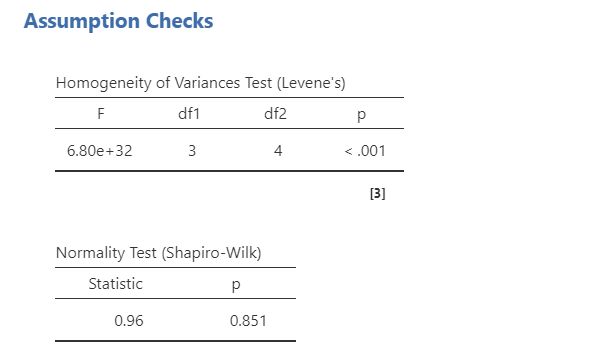
\includegraphics[width=1\linewidth]{images/06-factorial-anova/independent-factorial_assumptions} 

}

\caption{Assumption check results in jamovi}\label{fig:unnamed-chunk-1}
\end{figure}

Let's look at the main results next. We got three lines of results in addition to the typical residuals (error). The first two lines are our main effects of \texttt{attend} and \texttt{reading} on grades. The p-values for both are statistically significant indicating attend affects grades and reading affects grades. However, it also added an interaction term of \texttt{attend\ *\ reading}, which is not statistically significant. This means we do not have an interaction between attend and reading on grades. Interactions will be discussed in more detail in the next section.

\begin{figure}

{\centering 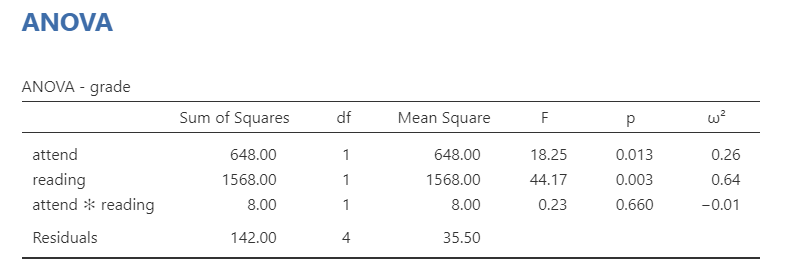
\includegraphics[width=1\linewidth]{images/06-factorial-anova/independent-factorial_results} 

}

\caption{Independent factorial ANOVA results in jamovi}\label{fig:unnamed-chunk-2}
\end{figure}

Although we could simply look at the means to know whether attending or reading had higher grades than not attending or not reading because there are only two conditions, we can also look at the post hoc tests and definitely need to look at them if we have three or more conditions per IV. These are shown below. Because the mean differences are negative, we can determine that the second group had higher means than the second group. We can confirm that with the estimated marginal means (not shown here).

\begin{figure}

{\centering 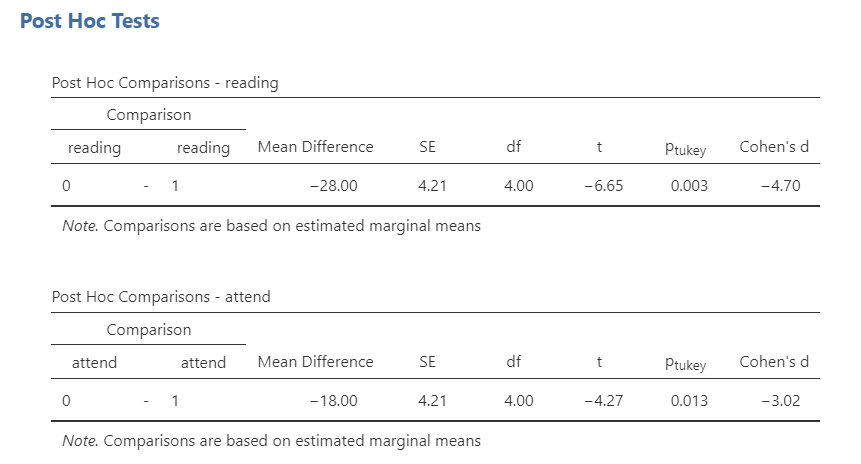
\includegraphics[width=1\linewidth]{images/06-factorial-anova/independent-factorial_posthoc} 

}

\caption{Post hoc results in jamovi}\label{fig:unnamed-chunk-3}
\end{figure}

Last, we can write-up our results!

\begin{quote}
We were interested in knowing how attendance and reading affected student grades. An independent factorial ANOVA showed that both attendance (\emph{F} {[}1, 4{]} = 18.25, \emph{p} = .013, \(\omega^2\) = .26) and reading (\emph{F} {[}1, 4{]} = 44.17, \emph{p} = .003, \(\omega^2\) = .64) affected student grades; there was no significant interaction between attendance and reading (\emph{F} {[}1, 4{]} = 8.00, \emph{p} = .660, \(\omega^2\) = -.01). Post hoc comparisons using Tukey's HSD show that students who attended lectures (\emph{M} = 75.50, \emph{SE} = 2.98) had higher grades than students who did not (\emph{M}~= 57.50, \emph{SE} = 2.98; \emph{p} = .003, \emph{d} = 4.70); furthermore, students who read (\emph{M} = 80.50, \emph{SE} = 2.98) had higher grades than students who did not (\emph{M} = 52.50, \emph{SE} = 2.98; \emph{p} = .013; \emph{d} = 3.02).
\end{quote}

\hypertarget{interactions}{%
\subsection{Interactions}\label{interactions}}

Interactions occur when the effect of one IV on the DV depends on the lvel of the other IV. If you did not want to test for interaction effects, you could remove them from the Model Terms in the Model drop-down menu.

However, by default they will include them. If you have 2-3 IVs, it may be reasonable to look at these interactions. However, 3-variable interactions (e.g., IV1 * IV2 * IV3) are pushing it and 4-variable interactions are highly implausible. Be critical in which interaction terms you include!

jamovi can provide a plot of your interaction, which can be helpful to help interpret your results. Below is the plot for our interaction of attendance on reading.

\begin{figure}

{\centering 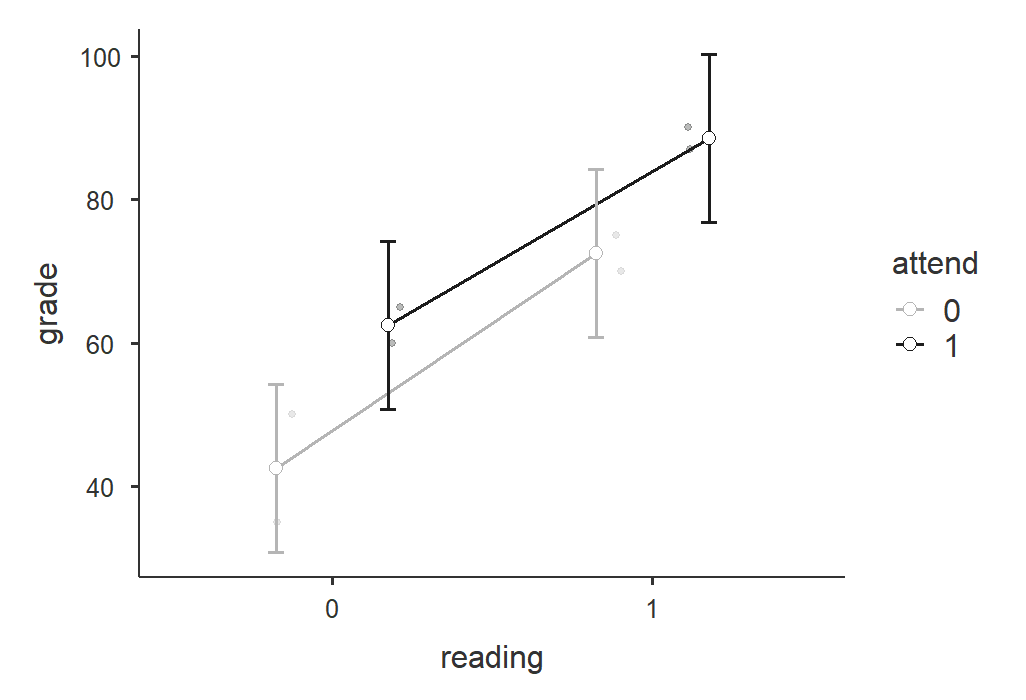
\includegraphics[width=1\linewidth]{images/06-factorial-anova/independent-factorial_plot} 

}

\caption{Interaction plot in jamovi}\label{fig:unnamed-chunk-4}
\end{figure}

The parallel lines that are sloping upward tell me there is a significant main effect for both IVs but no interaction. How do I know that? With two variables, there are only so many interaction shapes possible. \href{https://courses.washington.edu/smartpsy/interactions.htm}{This website} does a fantastic time showing you all 8 combinations of the three effects (2 main effects and 1 interaction effect). Spend some time looking through it and familiarizing yourself with the plots!

\hypertarget{repeated-measures-factorial-anova}{%
\section{Repeated Measures Factorial ANOVA}\label{repeated-measures-factorial-anova}}

This is also sometimes called the two-way (or three-way or n-way, depending on the \emph{n} of IVs you have) repeated measures ANOVA. Let's go through an example repeated measures factorial ANOVA. The dataset is courtesy of \href{https://www.real-statistics.com/anova-repeated-measures/two-within-subjects-factors/}{Real Statistics Using Excel}.

\begin{quote}
A company has created a new training program for their customer service staff. To test the effectiveness of the program they took a sample of 10 employees and assessed their performance in three areas: ~Product (knowledge of the company's products and services), Client (their ability to relate to the customer with politeness and empathy) and Action (their ability to take action to help the customer). They then had the same 10 employees take the training course and rated their performance after the program in the same three areas. -\href{A\%20company\%20has\%20created\%20a\%20new\%20training\%20program\%20for\%20their\%20customer\%20service\%20staff.\%20To\%20test\%20the\%20effectiveness\%20of\%20the\%20program\%20they\%20took\%20a\%20sample\%20of\%2010\%20employees\%20and\%20assessed\%20their\%20performance\%20in\%20three\%20areas:\%20Product\%20(knowledge\%20of\%20the\%20company’s\%20products\%20and\%20services),\%20Client\%20(their\%20ability\%20to\%20relate\%20to\%20the\%20customer\%20with\%20politeness\%20and\%20empathy)\%20and\%20Action\%20(their\%20ability\%20to\%20take\%20action\%20to\%20help\%20the\%20customer).\%20They\%20then\%20had\%20the\%20same\%2010\%20employees\%20take\%20the\%20training\%20course\%20and\%20rated\%20their\%20performance\%20after\%20the\%20program\%20in\%20the\%20same\%20three\%20areas.\%20Based\%20on\%20the\%20data\%20in\%20Figure\%201,\%20determine\%20whether\%20the\%20program\%20was\%20effective.}{Real Statistics Using Excel}
\end{quote}

\begin{longtable}[]{@{}lllllll@{}}
\caption{Dataset for the repeated measures factorial ANOVA}\tabularnewline
\toprule
\begin{minipage}[b]{0.05\columnwidth}\raggedright
ID\strut
\end{minipage} & \begin{minipage}[b]{0.13\columnwidth}\raggedright
Pre-Product\strut
\end{minipage} & \begin{minipage}[b]{0.12\columnwidth}\raggedright
Pre-Client\strut
\end{minipage} & \begin{minipage}[b]{0.12\columnwidth}\raggedright
Pre-Action\strut
\end{minipage} & \begin{minipage}[b]{0.14\columnwidth}\raggedright
Post-Product\strut
\end{minipage} & \begin{minipage}[b]{0.13\columnwidth}\raggedright
Post-Client\strut
\end{minipage} & \begin{minipage}[b]{0.13\columnwidth}\raggedright
Post-Action\strut
\end{minipage}\tabularnewline
\midrule
\endfirsthead
\toprule
\begin{minipage}[b]{0.05\columnwidth}\raggedright
ID\strut
\end{minipage} & \begin{minipage}[b]{0.13\columnwidth}\raggedright
Pre-Product\strut
\end{minipage} & \begin{minipage}[b]{0.12\columnwidth}\raggedright
Pre-Client\strut
\end{minipage} & \begin{minipage}[b]{0.12\columnwidth}\raggedright
Pre-Action\strut
\end{minipage} & \begin{minipage}[b]{0.14\columnwidth}\raggedright
Post-Product\strut
\end{minipage} & \begin{minipage}[b]{0.13\columnwidth}\raggedright
Post-Client\strut
\end{minipage} & \begin{minipage}[b]{0.13\columnwidth}\raggedright
Post-Action\strut
\end{minipage}\tabularnewline
\midrule
\endhead
\begin{minipage}[t]{0.05\columnwidth}\raggedright
1\strut
\end{minipage} & \begin{minipage}[t]{0.13\columnwidth}\raggedright
13\strut
\end{minipage} & \begin{minipage}[t]{0.12\columnwidth}\raggedright
12\strut
\end{minipage} & \begin{minipage}[t]{0.12\columnwidth}\raggedright
17\strut
\end{minipage} & \begin{minipage}[t]{0.14\columnwidth}\raggedright
18\strut
\end{minipage} & \begin{minipage}[t]{0.13\columnwidth}\raggedright
30\strut
\end{minipage} & \begin{minipage}[t]{0.13\columnwidth}\raggedright
34\strut
\end{minipage}\tabularnewline
\begin{minipage}[t]{0.05\columnwidth}\raggedright
2\strut
\end{minipage} & \begin{minipage}[t]{0.13\columnwidth}\raggedright
12\strut
\end{minipage} & \begin{minipage}[t]{0.12\columnwidth}\raggedright
19\strut
\end{minipage} & \begin{minipage}[t]{0.12\columnwidth}\raggedright
18\strut
\end{minipage} & \begin{minipage}[t]{0.14\columnwidth}\raggedright
6\strut
\end{minipage} & \begin{minipage}[t]{0.13\columnwidth}\raggedright
18\strut
\end{minipage} & \begin{minipage}[t]{0.13\columnwidth}\raggedright
30\strut
\end{minipage}\tabularnewline
\begin{minipage}[t]{0.05\columnwidth}\raggedright
3\strut
\end{minipage} & \begin{minipage}[t]{0.13\columnwidth}\raggedright
17\strut
\end{minipage} & \begin{minipage}[t]{0.12\columnwidth}\raggedright
19\strut
\end{minipage} & \begin{minipage}[t]{0.12\columnwidth}\raggedright
24\strut
\end{minipage} & \begin{minipage}[t]{0.14\columnwidth}\raggedright
21\strut
\end{minipage} & \begin{minipage}[t]{0.13\columnwidth}\raggedright
31\strut
\end{minipage} & \begin{minipage}[t]{0.13\columnwidth}\raggedright
32\strut
\end{minipage}\tabularnewline
\begin{minipage}[t]{0.05\columnwidth}\raggedright
4\strut
\end{minipage} & \begin{minipage}[t]{0.13\columnwidth}\raggedright
12\strut
\end{minipage} & \begin{minipage}[t]{0.12\columnwidth}\raggedright
25\strut
\end{minipage} & \begin{minipage}[t]{0.12\columnwidth}\raggedright
25\strut
\end{minipage} & \begin{minipage}[t]{0.14\columnwidth}\raggedright
18\strut
\end{minipage} & \begin{minipage}[t]{0.13\columnwidth}\raggedright
39\strut
\end{minipage} & \begin{minipage}[t]{0.13\columnwidth}\raggedright
40\strut
\end{minipage}\tabularnewline
\begin{minipage}[t]{0.05\columnwidth}\raggedright
5\strut
\end{minipage} & \begin{minipage}[t]{0.13\columnwidth}\raggedright
19\strut
\end{minipage} & \begin{minipage}[t]{0.12\columnwidth}\raggedright
27\strut
\end{minipage} & \begin{minipage}[t]{0.12\columnwidth}\raggedright
19\strut
\end{minipage} & \begin{minipage}[t]{0.14\columnwidth}\raggedright
18\strut
\end{minipage} & \begin{minipage}[t]{0.13\columnwidth}\raggedright
28\strut
\end{minipage} & \begin{minipage}[t]{0.13\columnwidth}\raggedright
27\strut
\end{minipage}\tabularnewline
\begin{minipage}[t]{0.05\columnwidth}\raggedright
6\strut
\end{minipage} & \begin{minipage}[t]{0.13\columnwidth}\raggedright
6\strut
\end{minipage} & \begin{minipage}[t]{0.12\columnwidth}\raggedright
12\strut
\end{minipage} & \begin{minipage}[t]{0.12\columnwidth}\raggedright
6\strut
\end{minipage} & \begin{minipage}[t]{0.14\columnwidth}\raggedright
6\strut
\end{minipage} & \begin{minipage}[t]{0.13\columnwidth}\raggedright
18\strut
\end{minipage} & \begin{minipage}[t]{0.13\columnwidth}\raggedright
23\strut
\end{minipage}\tabularnewline
\begin{minipage}[t]{0.05\columnwidth}\raggedright
7\strut
\end{minipage} & \begin{minipage}[t]{0.13\columnwidth}\raggedright
17\strut
\end{minipage} & \begin{minipage}[t]{0.12\columnwidth}\raggedright
18\strut
\end{minipage} & \begin{minipage}[t]{0.12\columnwidth}\raggedright
30\strut
\end{minipage} & \begin{minipage}[t]{0.14\columnwidth}\raggedright
24\strut
\end{minipage} & \begin{minipage}[t]{0.13\columnwidth}\raggedright
36\strut
\end{minipage} & \begin{minipage}[t]{0.13\columnwidth}\raggedright
38\strut
\end{minipage}\tabularnewline
\begin{minipage}[t]{0.05\columnwidth}\raggedright
8\strut
\end{minipage} & \begin{minipage}[t]{0.13\columnwidth}\raggedright
18\strut
\end{minipage} & \begin{minipage}[t]{0.12\columnwidth}\raggedright
29\strut
\end{minipage} & \begin{minipage}[t]{0.12\columnwidth}\raggedright
36\strut
\end{minipage} & \begin{minipage}[t]{0.14\columnwidth}\raggedright
22\strut
\end{minipage} & \begin{minipage}[t]{0.13\columnwidth}\raggedright
36\strut
\end{minipage} & \begin{minipage}[t]{0.13\columnwidth}\raggedright
40\strut
\end{minipage}\tabularnewline
\begin{minipage}[t]{0.05\columnwidth}\raggedright
9\strut
\end{minipage} & \begin{minipage}[t]{0.13\columnwidth}\raggedright
23\strut
\end{minipage} & \begin{minipage}[t]{0.12\columnwidth}\raggedright
30\strut
\end{minipage} & \begin{minipage}[t]{0.12\columnwidth}\raggedright
24\strut
\end{minipage} & \begin{minipage}[t]{0.14\columnwidth}\raggedright
18\strut
\end{minipage} & \begin{minipage}[t]{0.13\columnwidth}\raggedright
38\strut
\end{minipage} & \begin{minipage}[t]{0.13\columnwidth}\raggedright
32\strut
\end{minipage}\tabularnewline
\begin{minipage}[t]{0.05\columnwidth}\raggedright
10\strut
\end{minipage} & \begin{minipage}[t]{0.13\columnwidth}\raggedright
18\strut
\end{minipage} & \begin{minipage}[t]{0.12\columnwidth}\raggedright
12\strut
\end{minipage} & \begin{minipage}[t]{0.12\columnwidth}\raggedright
24\strut
\end{minipage} & \begin{minipage}[t]{0.14\columnwidth}\raggedright
24\strut
\end{minipage} & \begin{minipage}[t]{0.13\columnwidth}\raggedright
25\strut
\end{minipage} & \begin{minipage}[t]{0.13\columnwidth}\raggedright
34\strut
\end{minipage}\tabularnewline
\bottomrule
\end{longtable}

You can copy-paste the table into Microsoft Excel, save as an .xlsx or .csv file, and import into jamovi to follow-along.

In jamovi, select Repeated Measures ANOVA under the ANOVA analysis option. Here are the general steps:

\begin{enumerate}
\def\labelenumi{\arabic{enumi}.}
\item
  In Repeated Measures Factors, you'll need to name both factors. Rename \texttt{RM\ Factor\ 1} to Time and \texttt{RM\ Factor\ 2} to Area. Under Time, specify two levels: Pre and Post. Under Area, specify three levels: Product, Client, and Action.
\item
  In Repeated Measures Cells, you'll now have six cells with the combinations of the 6 columns you have. Drag the variable from the left into the correct cell on the right. Be careful here! For example, you need to put the Pre-Product variable into the cell ``Pre, Product''.
\item
  Name your dependent variable label ``Performance'' and select `Generalised \(\eta^2\).
\item
  Under Assumption Checks, select Sphericity tests
\item
  Under Post Hoc Tests, move Area and Time over and select Tukey.
\item
  Under Estimated Marginal Means, move Time over into Term 1, Area into Term 2, and both Time and Area into Term 3. Select plots and tables, Observed scores, and Equal cell weights.
\end{enumerate}

Now let's go over selected output. First, we need to check our assumption of sphericity. All the Mauchly's W's are not statistically significant so we satisfy the assumption of sphericity and do not need to apply any sphericity corrections.

\begin{figure}

{\centering 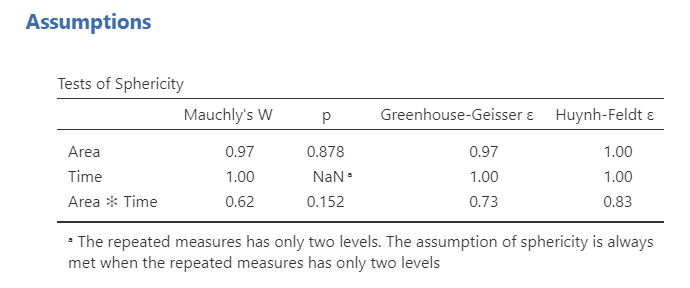
\includegraphics[width=1\linewidth]{images/06-factorial-anova/rm-factorial_assumption} 

}

\caption{Assumption testing in jamovi}\label{fig:unnamed-chunk-5}
\end{figure}

Next let's look at the within subjects effects table. Remember, we do not need to worry about the between subjects effects table because we do not have one; it will be used in the mixed factorial design below. Overall, we see a significant main effect of area, a significant main effect of time, and a significant interaction effect of both area and time. Neat!

\begin{figure}

{\centering 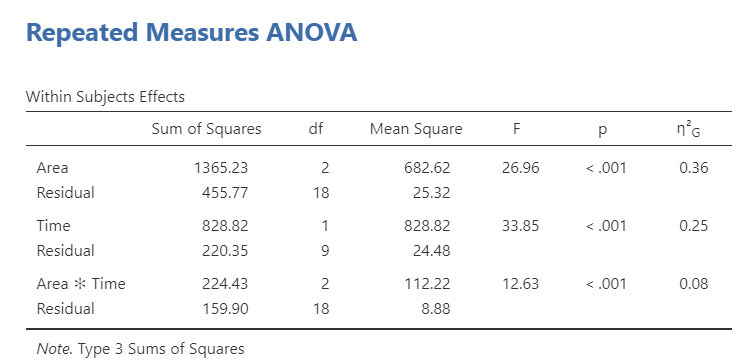
\includegraphics[width=1\linewidth]{images/06-factorial-anova/rm-factorial_results} 

}

\caption{Repeated measures ANOVA in jamovi}\label{fig:unnamed-chunk-6}
\end{figure}

Next, we can look at post hoc comparisons because the main effects were all statistically significant. For area, we can see that client and action had significantly higher means than product, but there was no difference between client and action. Furthermore, post-intervention performance was significantly higher than pre-intervention.

\begin{figure}

{\centering 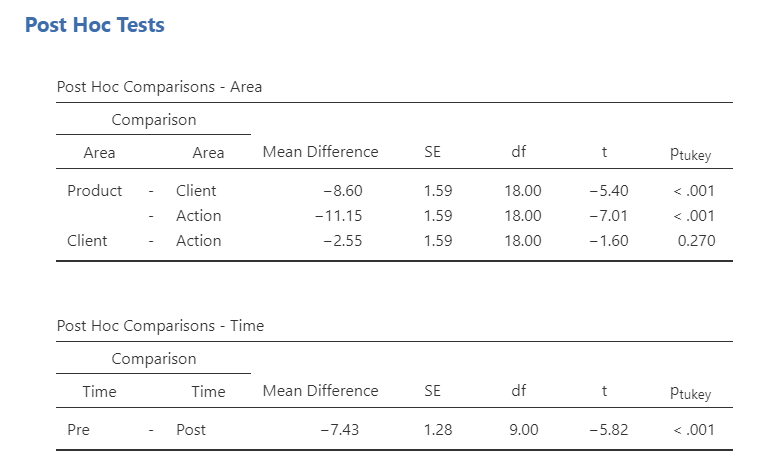
\includegraphics[width=1\linewidth]{images/06-factorial-anova/rm-factorial_tukey} 

}

\caption{Post hoc tests in jamovi}\label{fig:unnamed-chunk-7}
\end{figure}

Last, let's look at the interaction to get a sense of what the interaction looks like. It appears that although there are no differences between pre- and post-intervention for product, there are significant differences from pre- to post-intervention for both client and action. To be more specific on where the statistically significant differences are, you can also ask for post hoc tests for the interaction term. This is where including a plot can be very helpful for your audience!

\begin{figure}

{\centering 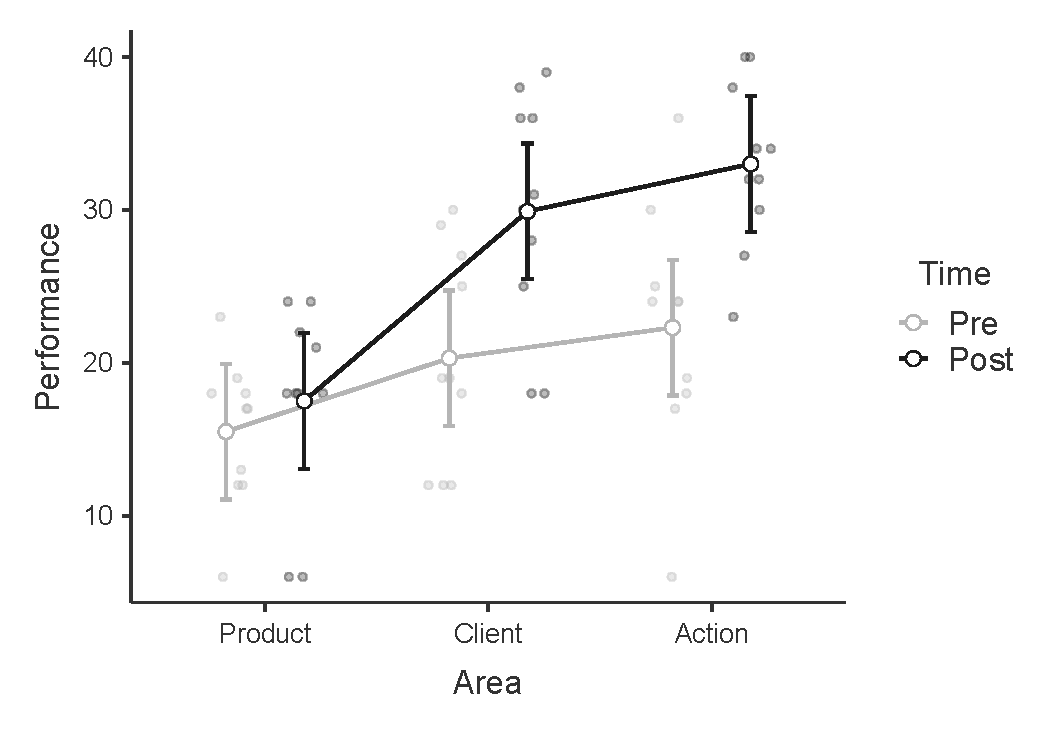
\includegraphics[width=1\linewidth]{images/06-factorial-anova/rm-factorial_interaction} 

}

\caption{Interaction plot in jamovi}\label{fig:unnamed-chunk-8}
\end{figure}

Now we have everything we need (in addition to the estimated marginal means) and can write-up our results.

\begin{quote}
We tested a 2 (time: pre- and post-intervention) x 3 (area: product, client, action) repeated measures factorial design to examine how both time and area affected performance. We satisfied the assumption of sphericity for all effects. There was a significant main effect of time (\emph{F} {[}1, 9{]} = 33.85, \emph{p} \textless{} .001, \(\eta^2_G\) = .25) such that performance at post-intervention (\emph{M} = 26.80, \emph{SE} = 1.84) was higher than at pre-intervention (\emph{M} = 19.37, \emph{SE} = 1.84). There was also a significant main effect of area (\emph{F} {[}2, 18{]} = 26.96, \emph{p} \textless{} .001, \(\eta^2_G\) = .36) such that both client (\emph{M} = 25.10, \emph{SE} = 1.95) and action (\emph{M} = 27.65, \emph{SE}~= 19.5) performance was higher than product performance (\emph{M} = 16.50, \emph{SE} = 1.95), but there was no difference between client and action performance. Lastly, there was a significant interaction between time and area such that there were no differences in product performance from pre- to post-intervention but there was for client and action performance (see Figure 1).
\end{quote}

\hypertarget{mixed-factorial-anova}{%
\section{Mixed Factorial ANOVA}\label{mixed-factorial-anova}}

Download the data for this analysis here:

This dataset comes from a larger studying examining the effect of a delayed reward preference of three commodities (food, money, and music) on food cravings (as rated by the Food Craving Questionnaire {[}FCQ{]}) for each participant. Participants were in one of two conditions: the control condition did not do anything and the experimental condition had participants do the tasks while fasting.

Therefore, this study is a 2 (between-subjects: condition {[}control or fasting{]}) x 3 (within-subjects: reward {[}food, money, and music{]}) mixed factorial design.

To perform a mixed factorial ANOVA, we use the same procedures as the repeated measures ANOVA but we also need to add a between-subjects factor.

\begin{enumerate}
\def\labelenumi{\arabic{enumi}.}
\item
  To perform a mixed factorial ANOVA in jamovi, go to the Analyses tab, click the ANOVA button, and choose ``Repeated Measures ANOVA''.
\item
  Under ``Repeated Measures Factors'' name your independent variable. In this case you can name it ``Reward''. Rename the three levels of Task: Food, Money, and Music.
\item
  Under ``Repeated Measures Cells'' move the given variable into the correct level. For example, you'll move FQ\_1 to Food, FQ\_2 to Money, and FQ\_3 to Music.
\item
  Under ``Between Subject Factors'' add your between-subjects variable "condition.
\item
  Select Generalised \(\eta^2\) as your measure of effect size.
\item
  In the Assumption Checks drop-down menu, select \texttt{Sphericity\ tests}.
\item
  In the Post Hoc Tests drop-down menu, move your two independent variables over and select \texttt{Tukey}. Remember that we only interpret these if the overall \emph{F} is statistically significant.
\item
  In the Estimated Marginal Means drop-down menu, move Reward, Condition, and both reward and condition into the terms under Marginal Means. Select tables and plots, and select \texttt{Observed\ scores}. Uncheck \texttt{Equal\ cell\ weights}.
\end{enumerate}

Now let's go through the output!

First, as always we check our assumption of sphericity. Mauchly's W is not statistically significant (\emph{p} = .073) so we satisfy the assumption of sphericity. We do not need to apply a sphericity correction.

\begin{figure}

{\centering 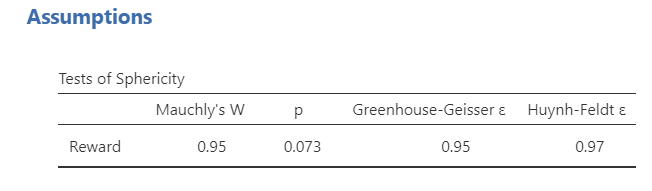
\includegraphics[width=1\linewidth]{images/06-factorial-anova/mixed_assumptions} 

}

\caption{Assumption checking in jamovi}\label{fig:unnamed-chunk-9}
\end{figure}

Next, we interpret out output! This time we interpret both our within subjects effects and between subjects effects tables. In the within subjects effects table, our main effect of reward is statistically significant. In the between subjects effects table, our main effect of condition is statistically significant. However, in the within subjects effects table, there is no statistically significant interaction effect of reward on condition.

\begin{figure}

{\centering 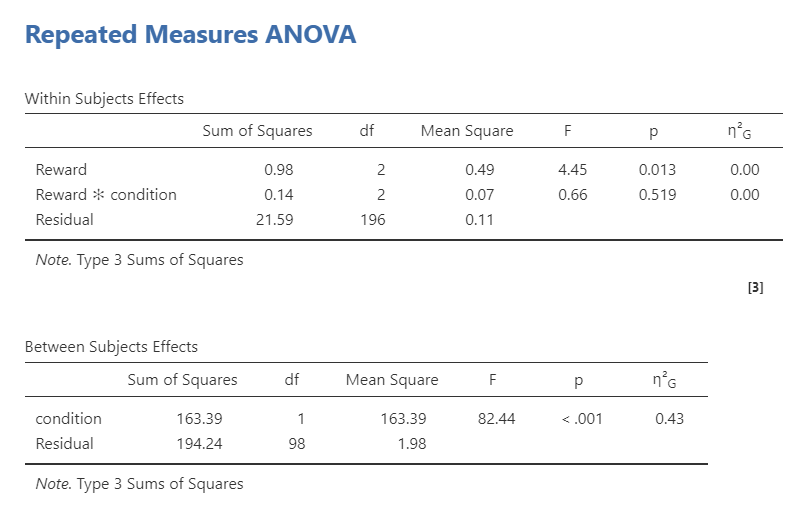
\includegraphics[width=1\linewidth]{images/06-factorial-anova/mixed_results} 

}

\caption{Mixed factorial ANOVA in jamovi}\label{fig:unnamed-chunk-10}
\end{figure}

To understand where the differences lie between conditions or reward preferences, we look to our post hoc tests. For reward, it looks like there is only a significant difference between food and music (\emph{p} = .009). For condition, it looks like cravings were higher in the fasting group than in the control group. We can look at the estimated marginal means tables to find the actual Means of the conditions and see the plots.

\begin{figure}

{\centering 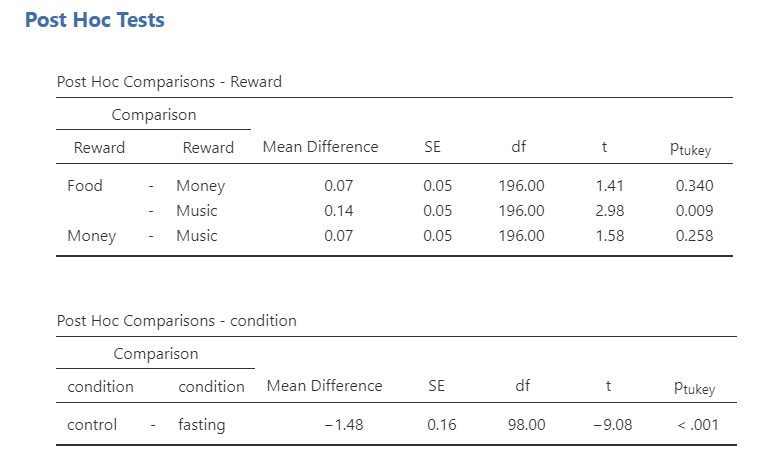
\includegraphics[width=1\linewidth]{images/06-factorial-anova/mixed_posthoc} 

}

\caption{Post hoc tests in jamovi}\label{fig:unnamed-chunk-11}
\end{figure}

We can look at the interaction plot, but notice that the lines are parallel which is a good indication that there is no significant interaction.

\begin{figure}

{\centering 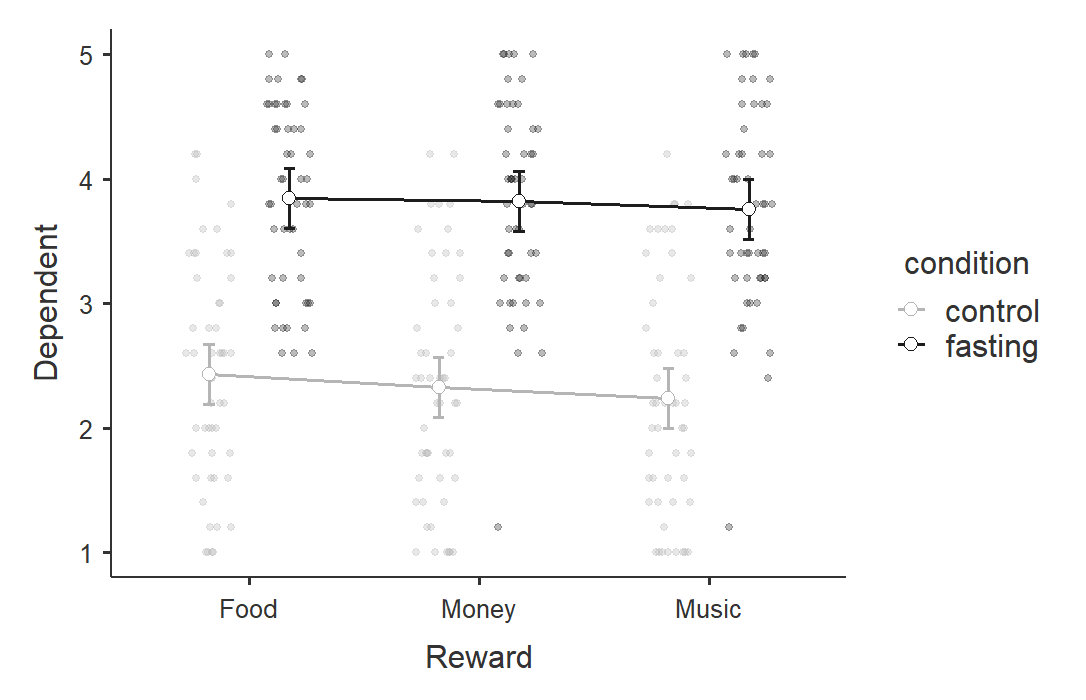
\includegraphics[width=1\linewidth]{images/06-factorial-anova/mixed_interaction} 

}

\caption{Interaction plot in jamovi}\label{fig:unnamed-chunk-12}
\end{figure}

Lastly, we can write up the results in APA style!

\begin{quote}
To test how both condition (control or fasting) and reward preference (food, money, and music) affected food cravings, we performed a mixed factorial ANOVA. There was a significant main effect of condition (\emph{F} {[}2, 196{]} = 4.45, \emph{p} = .013, \(\eta^2_G\) = .00) and a significant main effect of reward (\emph{F} {[}1, 98{]} = 82.44, \emph{p} \textless{} .001, \(\eta^2_G\) = .43). However, there was no statistically significant interaction effect of reward on condition (\emph{F} {[}2, 196{]} = .66, \emph{p} = .519, \(\eta^2_G\) = .00).

For condition, participants who fasted (\emph{M} = 3.81, \emph{SE} = .11) reported significantly more food cravings than participants in the control condition (\emph{M} = 2.33, \emph{SE} = .11; \(p_{Tukey}\) \textless{} .001). For reward, the food reward (\emph{M} = 3.14, \emph{SE} = .09) led to significantly higher food cravings than the music reward (\emph{M} = 3.00, \emph{SE} = .09; \(p_{Tukey}\) = .009), but there was no differences between the money reward (\emph{M} = 3.07, \emph{SE} = .09) and both food (\(p_{Tukey}\) = .340) or music (\(p_{Tukey}\) = .258).
\end{quote}

\hypertarget{ancova}{%
\chapter{ANCOVA}\label{ancova}}

\hypertarget{what-is-ancova}{%
\section{What is ANCOVA?}\label{what-is-ancova}}

\textbf{ANCOVA} (\textbf{AN}alysis of \textbf{COVA}riance) examines the difference in means between \underline{three or more} groups, while controlling for or partialling out the effect of one or more continuous confounds or covariates.

\textbf{Some definitions}: A \emph{confounding} variable is a variable that affects or is related to both the independent and dependent variable. A \emph{covariate} variable is a variable that only affects or is only related to the dependent variable.

There are two main reasons for including covariates:

\begin{enumerate}
\def\labelenumi{\arabic{enumi}.}
\item
  \textbf{To reduce within-group error variance}: Remember that to get a larger F-statistic, we need to maximize between-groups variance and minimize within-groups variance. Adding covariates can sometimes minimize within-groups variance if that covariate helps \emph{explain} some of the within-group variance.
\item
  \textbf{Elimination of covariates}: Sometimes there are other variables that also explain our outcome variable. We want to look at the effect of another variable on the outcome while removing or eliminating the other variables (confounds) that also explain our outcome variable.
\end{enumerate}

\hypertarget{assumptions-of-ancova}{%
\section{Assumptions of ANCOVA}\label{assumptions-of-ancova}}

In addition to the same assumptions of the one-way ANOVA (see \ref{anova-assumptions}), the ANCOVA has two additional assumptions:

\begin{enumerate}
\def\labelenumi{\arabic{enumi}.}
\item
  \textbf{Independence of the covariate and treatment effect}: When the covariate and treatment effect are related, then we can have incorrect F-statistic values. However, this is only important in experimental designs. In quasi-experimental designs, this is often violated and you just have to interpret results accordingly.

  \begin{itemize}
  \tightlist
  \item
    If you do have an experimental manipulation with a covariate, you can test this assumption by running a one-way ANOVA but with your experimental manipulation as your IV or group variable and your covariate as your DV. If there is a significant F-ratio, then you have violated this assumption.
  \end{itemize}
\item
  \textbf{Homogeneity of regression slopes}: The relationship between the covariate and the outcomes must be similar across groups.

  \begin{itemize}
  \tightlist
  \item
    To test this assumption, add an interaction term between the covariate and each independent variable in jamovi under the Model drop-down menu. Add the interactions as model terms.
  \end{itemize}
\end{enumerate}

\hypertarget{ancova-in-jamovi}{%
\section{ANCOVA in jamovi}\label{ancova-in-jamovi}}

Let's run an example with data from lsj-data. Open data from your Data Library in ``lsj-data''. Select and open ``ancova''. This data is fictional data from a health psychologist who was interested in the effect of routine cycling (1 = driving, 2 = cycling) and stress (1 = high, 2 = low) on happiness levels, with age as a covariate. Notice how this is a 2x2 independent factorial design with a covariate!

\begin{enumerate}
\def\labelenumi{\arabic{enumi}.}
\item
  To perform an ANCOVA in jamovi, select ANCOVA under the ANOVA analysis menu.
\item
  Move your dependent variable \texttt{happiness} to the Dependent Variable box, your independent variables \texttt{stress} and \texttt{commute} to the Fixed Factors box, and your covariate \texttt{age} to the Covariates box.
\item
  Select \(\omega^2\) as your effect size.
\item
  Under Assumption Checks, select all three assumption checks: \texttt{Homogeneity\ test}, \texttt{Normality\ test}, and \texttt{Q-Q\ Plot}.
\item
  Under Post Hoc Tests, move both of your independent variables over, select the \texttt{Tukey} correction and select \texttt{Cohen\textquotesingle{}s\ d} for your effect size.
\item
  Under Estimated Marginal Means, move each of your independent variables over into its own term box. Also include combinations of your independent variables if you have an interaction term in your model. Select both plots and tables, select \texttt{Observed\ scores}, and de-select \texttt{Equal\ cell\ weights}.
\end{enumerate}

First, let's check our assumptions in jamovi. Shapiro-Wilk's test was not statistically significant (\emph{p} = .735) and the Q-Q plot looks good; therefore, we've satisfied the assumption of normality. Levene's test was not statistically significant (\emph{p} = .925); therefore, we've satisfied the assumption of homogeneity of variance.

\begin{figure}

{\centering 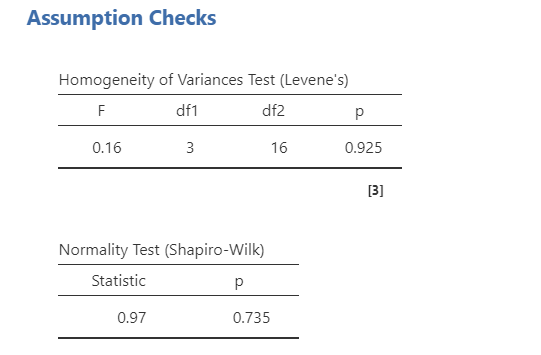
\includegraphics[width=1\linewidth]{images/07-ancova/ancova_assumptions} 

}

\caption{Assumption check results in jamovi}\label{fig:unnamed-chunk-1}
\end{figure}

However, we have two additional assumptions we need to check. Let's check the assumption of independence of the covariate and treatment effect. For that, we need to perform another ANOVA (not an ANCOVA) with our independent variables predicting age. Our results indicate we violate this assumption: both \texttt{stress} and the interaction of \texttt{stress\ *\ commute} are related to age. This suggests age is in fact a \emph{confounding} variable, not a covariate. We should be performing a mediation, but because we want to illustrate the ANCOVA we will continue.

\begin{figure}

{\centering 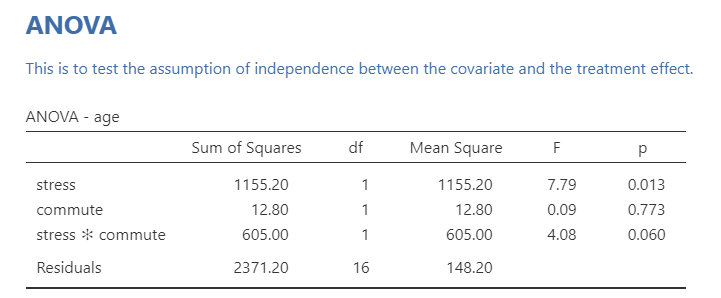
\includegraphics[width=1\linewidth]{images/07-ancova/ancova_assumptions2} 

}

\caption{Assumption check results in jamovi}\label{fig:unnamed-chunk-2}
\end{figure}

The second additional assumption is that the relationship between the covariate and the dependent variable is similar for all levels of the independent variable (homogeneity of regression slopes). We can test this by adding an interaction term between the covariate and each independent variable in jamovi under the Model drop-down menu. If the interaction effect is not significant it can be removed. If it is significant then a different and more advanced statistical technique might be appropriate (which is beyond the scope of this class). In our case, the interactions between each IV and our covariate are not statistically significant so we can remove the interaction terms and move on.

\begin{figure}

{\centering 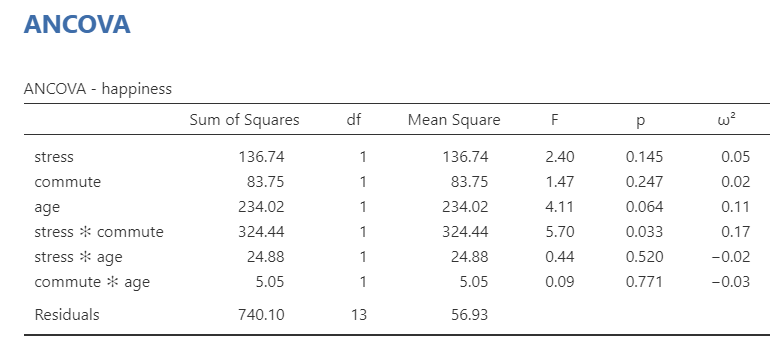
\includegraphics[width=1\linewidth]{images/07-ancova/ancova_assumptions3} 

}

\caption{Assumption check results in jamovi}\label{fig:unnamed-chunk-3}
\end{figure}

Now it's time to interpret the results! The ANCOVA table shows that both independent variables (\texttt{stress} and \texttt{commute}), the interaction term (\texttt{stress\ *\ commute*}), and the covariate (\texttt{age}) are statistically significant. Therefore, we can look at our post hoc tests to find where the differences are.

\begin{figure}

{\centering 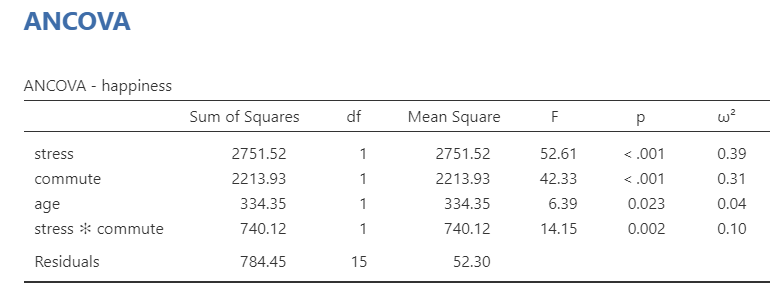
\includegraphics[width=1\linewidth]{images/07-ancova/ancova_results} 

}

\caption{ANCOVA results in jamovi}\label{fig:unnamed-chunk-4}
\end{figure}

\begin{info}
Technically, we don't need to look at the post hoc table much in this
example. Because there are only two groups, we already know one group
will have higher means than the other group if the F-test is
significant. In fact, check this out: the square root of our F-statistic
is equal to the t-statistic in our post hoc table. Neat!
\end{info}

Post hoc tests show that low stress had higher happiness than high stress, and that cycling had higher happiness than driving. We can also look to the estimated marginal means tables and plots for information for reporting.

\begin{figure}

{\centering 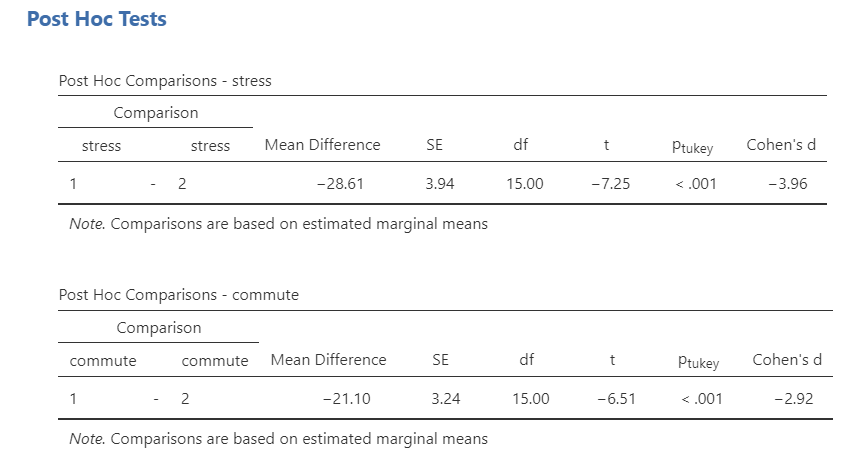
\includegraphics[width=1\linewidth]{images/07-ancova/ancova_tukey} 

}

\caption{Post hoc results in jamovi}\label{fig:unnamed-chunk-6}
\end{figure}

Last, we can write-up our results! Reporting ANCOVA is very similar to reporting an ANOVA test (in this case an independent factorial ANOVA) except that we also report the effect of the covariate, as well. Here's an example write-up:

\begin{quote}
We conducted a study examining how stress and commute affect happiness levels in a 2 (stress: high or low) x 2 (commute: cycling or driving) independent factorial design. Furthermore, we collected data on age as a covariate of our study. We satisfied all assumptions of the ANCOVA except that age was in fact a confounding variable in that it relates to our independent variable of stress. Despite failing to meet this assumption, we proceeded with the ANCOVA analysis.

There was a significant main effect of stress on happiness such that participants in the low stress condition (\emph{M} = 68.45, \emph{SE} = 2.55) reported significantly greater happiness than participants in the high stress condition (\emph{M} = 39.85, \emph{SE} = 2.55), \emph{F} (1, 15) = 52.61, \emph{p} \textless{} .001, \(\omega^2\) = .39. There was also a significant main effect of commute on happiness such that participants who commuted via cycling (\emph{M} = 64.70, \emph{SE} = 2.29) reported significantly greater happiness than participants who commuted via driving (\emph{M} = 43.60, \emph{SE} = 2.29), \emph{F} (1, 15) = 42.33, \emph{p} \textless{} .001, \(\omega^2\) = .31. There was a significant interaction between stress and commute type such that happiness levels were similar in the low stress condition for both commute types, but happiness was significantly higher for participants who cycled versus those who drove in the high stress condition, \emph{F} (1, 15) = 14.15, \emph{p}~= .002, \(\omega^2\) = .10. Furthermore, age was a significant covariate of our dependent variable, \emph{F} (1, 15) = 6.39, \emph{p} = .023, \(\omega^2\) = .04.
\end{quote}

\begin{figure}

{\centering \includegraphics[width=1\linewidth]{images/07-ancova/ancova_interaction} 

}

\caption{Interaction in jamovi}\label{fig:unnamed-chunk-7}
\end{figure}

\hypertarget{appendix-appendices}{%
\appendix}


\hypertarget{references}{%
\chapter{References}\label{references}}

  \bibliography{book.bib,packages.bib}

\end{document}
